\addtocontents{toc}{\protect\addvspace{5pt}}
\chapter{HASIL DAN PEMBAHASAN}

\section{Analisis Data Referensi SSFM}

Data referensi perambatan pulsa diperoleh melalui teknik numerik SSFM. Gambar \ref{fig:reference} menunjukkan adanya peningkatan daya maksimum pulsa diiringi oleh proses kompresi terhadap kondisi awal. Keseluruhan proses perambatan pulsa dipengaruhi oleh nilai dispersi kecepatan grup $\beta_2$ dan interaksinya terhadap nonlinearitas serat optik $\gamma$.


\begin{figure}[htbp]
    \centering
    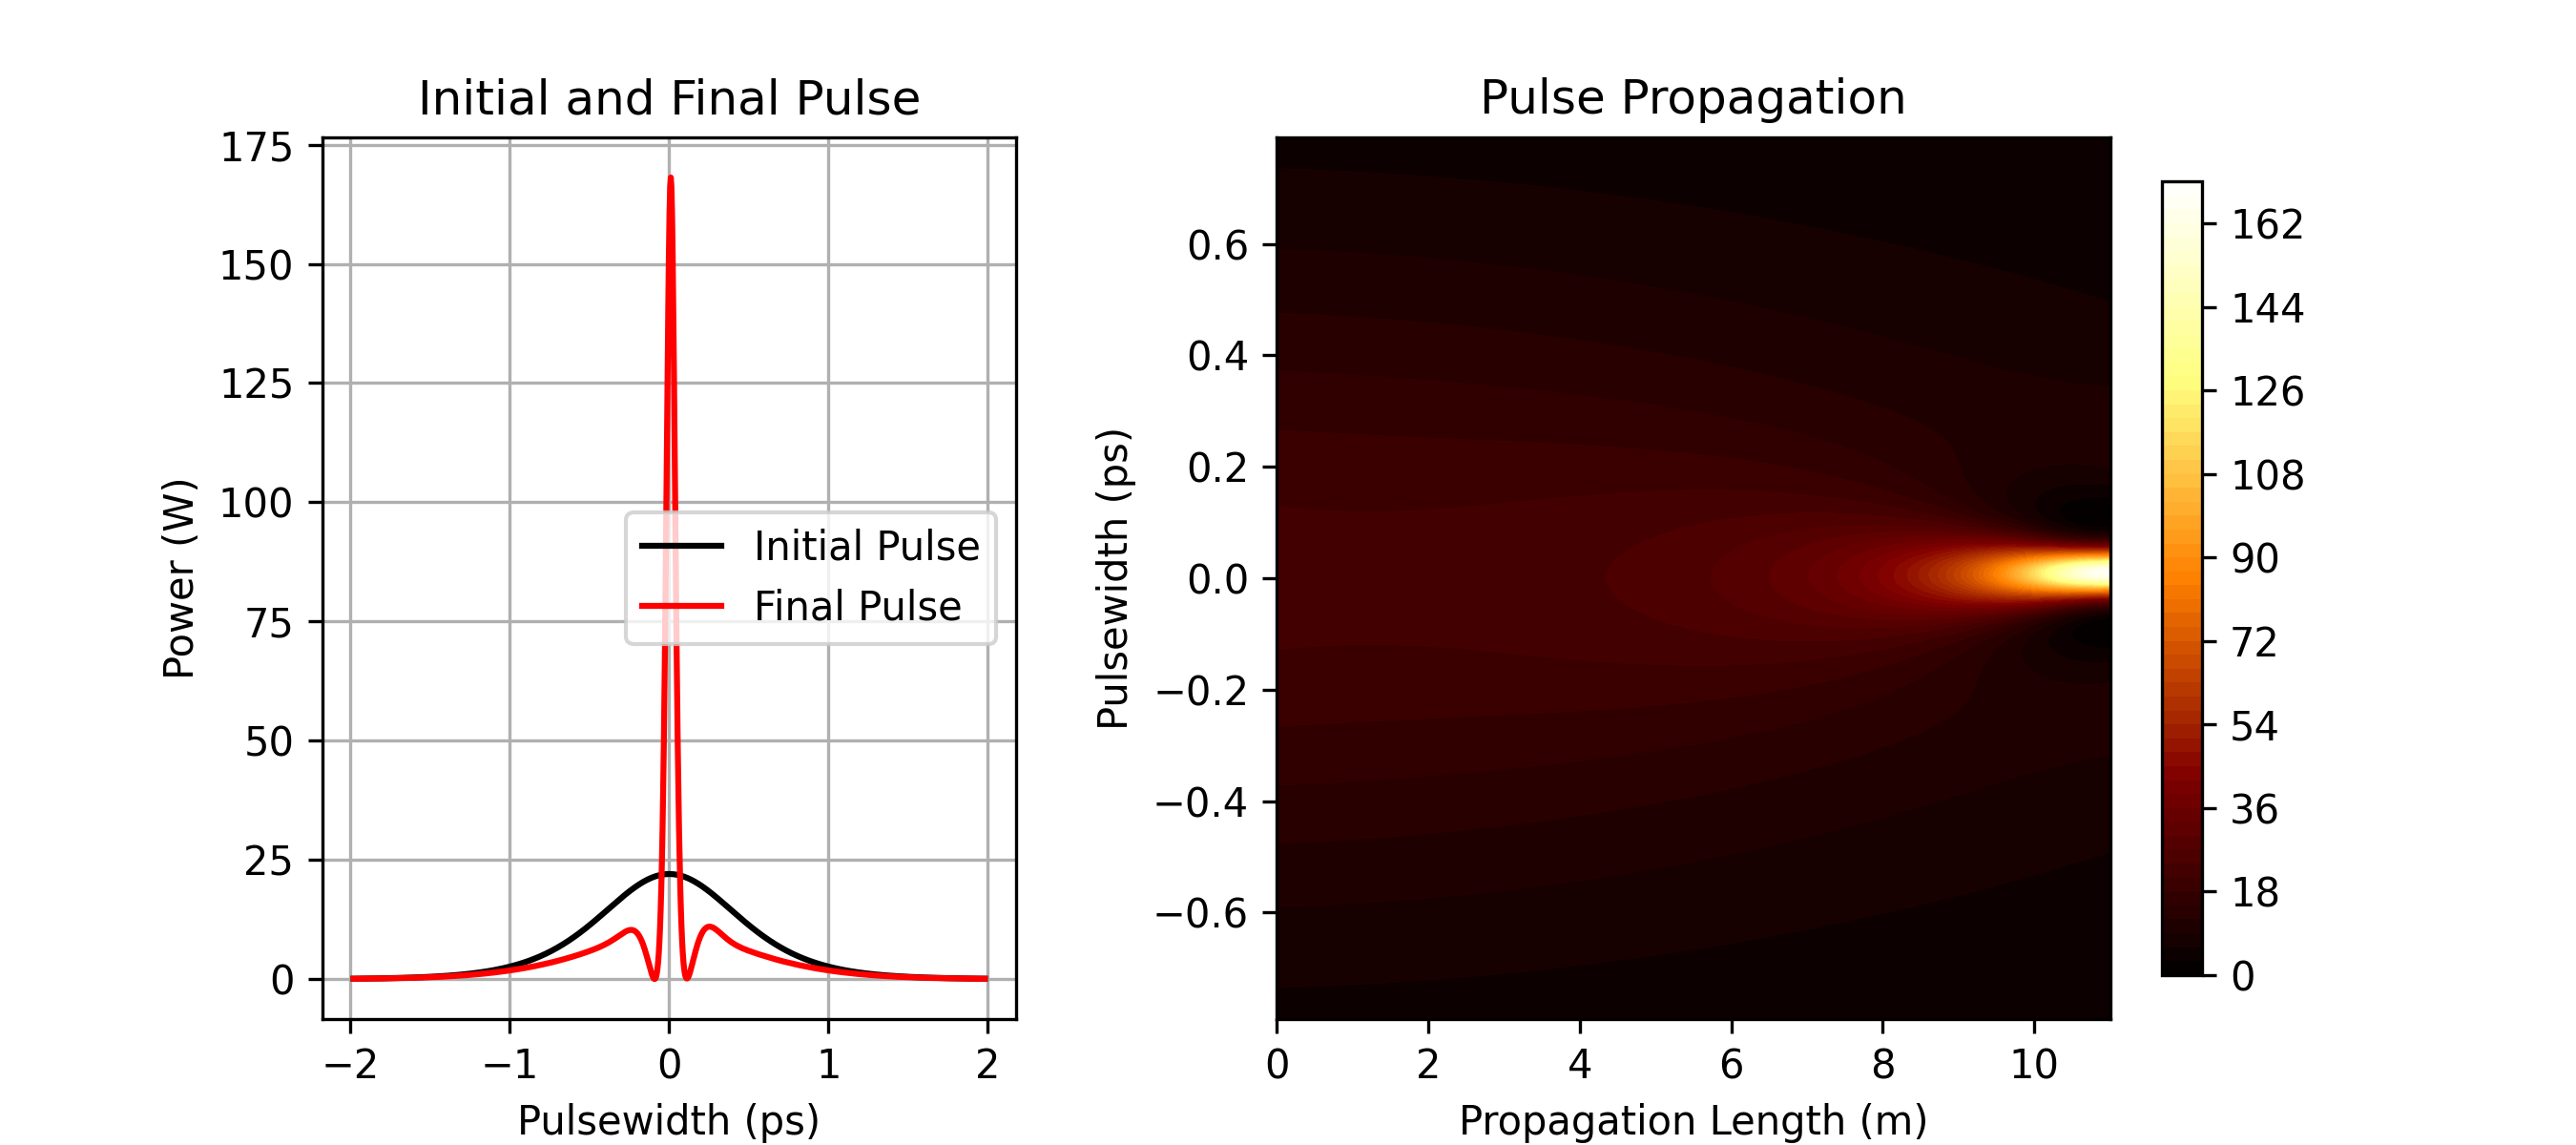
\includegraphics[width=1\linewidth]{Gambar/GroundTruth3D.png}
    \caption{Daya Pulsa Referensi (SSFM)}
    (a) Kondisi Awal dan Akhir; (b) Perambatan Pulsa
    \label{fig:reference}
\end{figure}

Nilai $\beta_2$ negatif menunjukkan sistem dispersi anomali di mana gelombang berfrekuensi tinggi bergerak lebih cepat. Hal ini menyebabkan terjadinya kompresi pulsa ketika efek dispersi mampu mengimbangi nonlinearitas serat optik. Sementara itu, orde dispersi ketiga $\beta_3$ menyatakan perubahan nilai dispersi kecepatan grup yang tidak dapat diabaikan pada sistem dengan lebar pulsa yang sangat pendek $T_0 < 1 \textbf{ ps}$.

\begin{figure}[htbp]
    \centering
    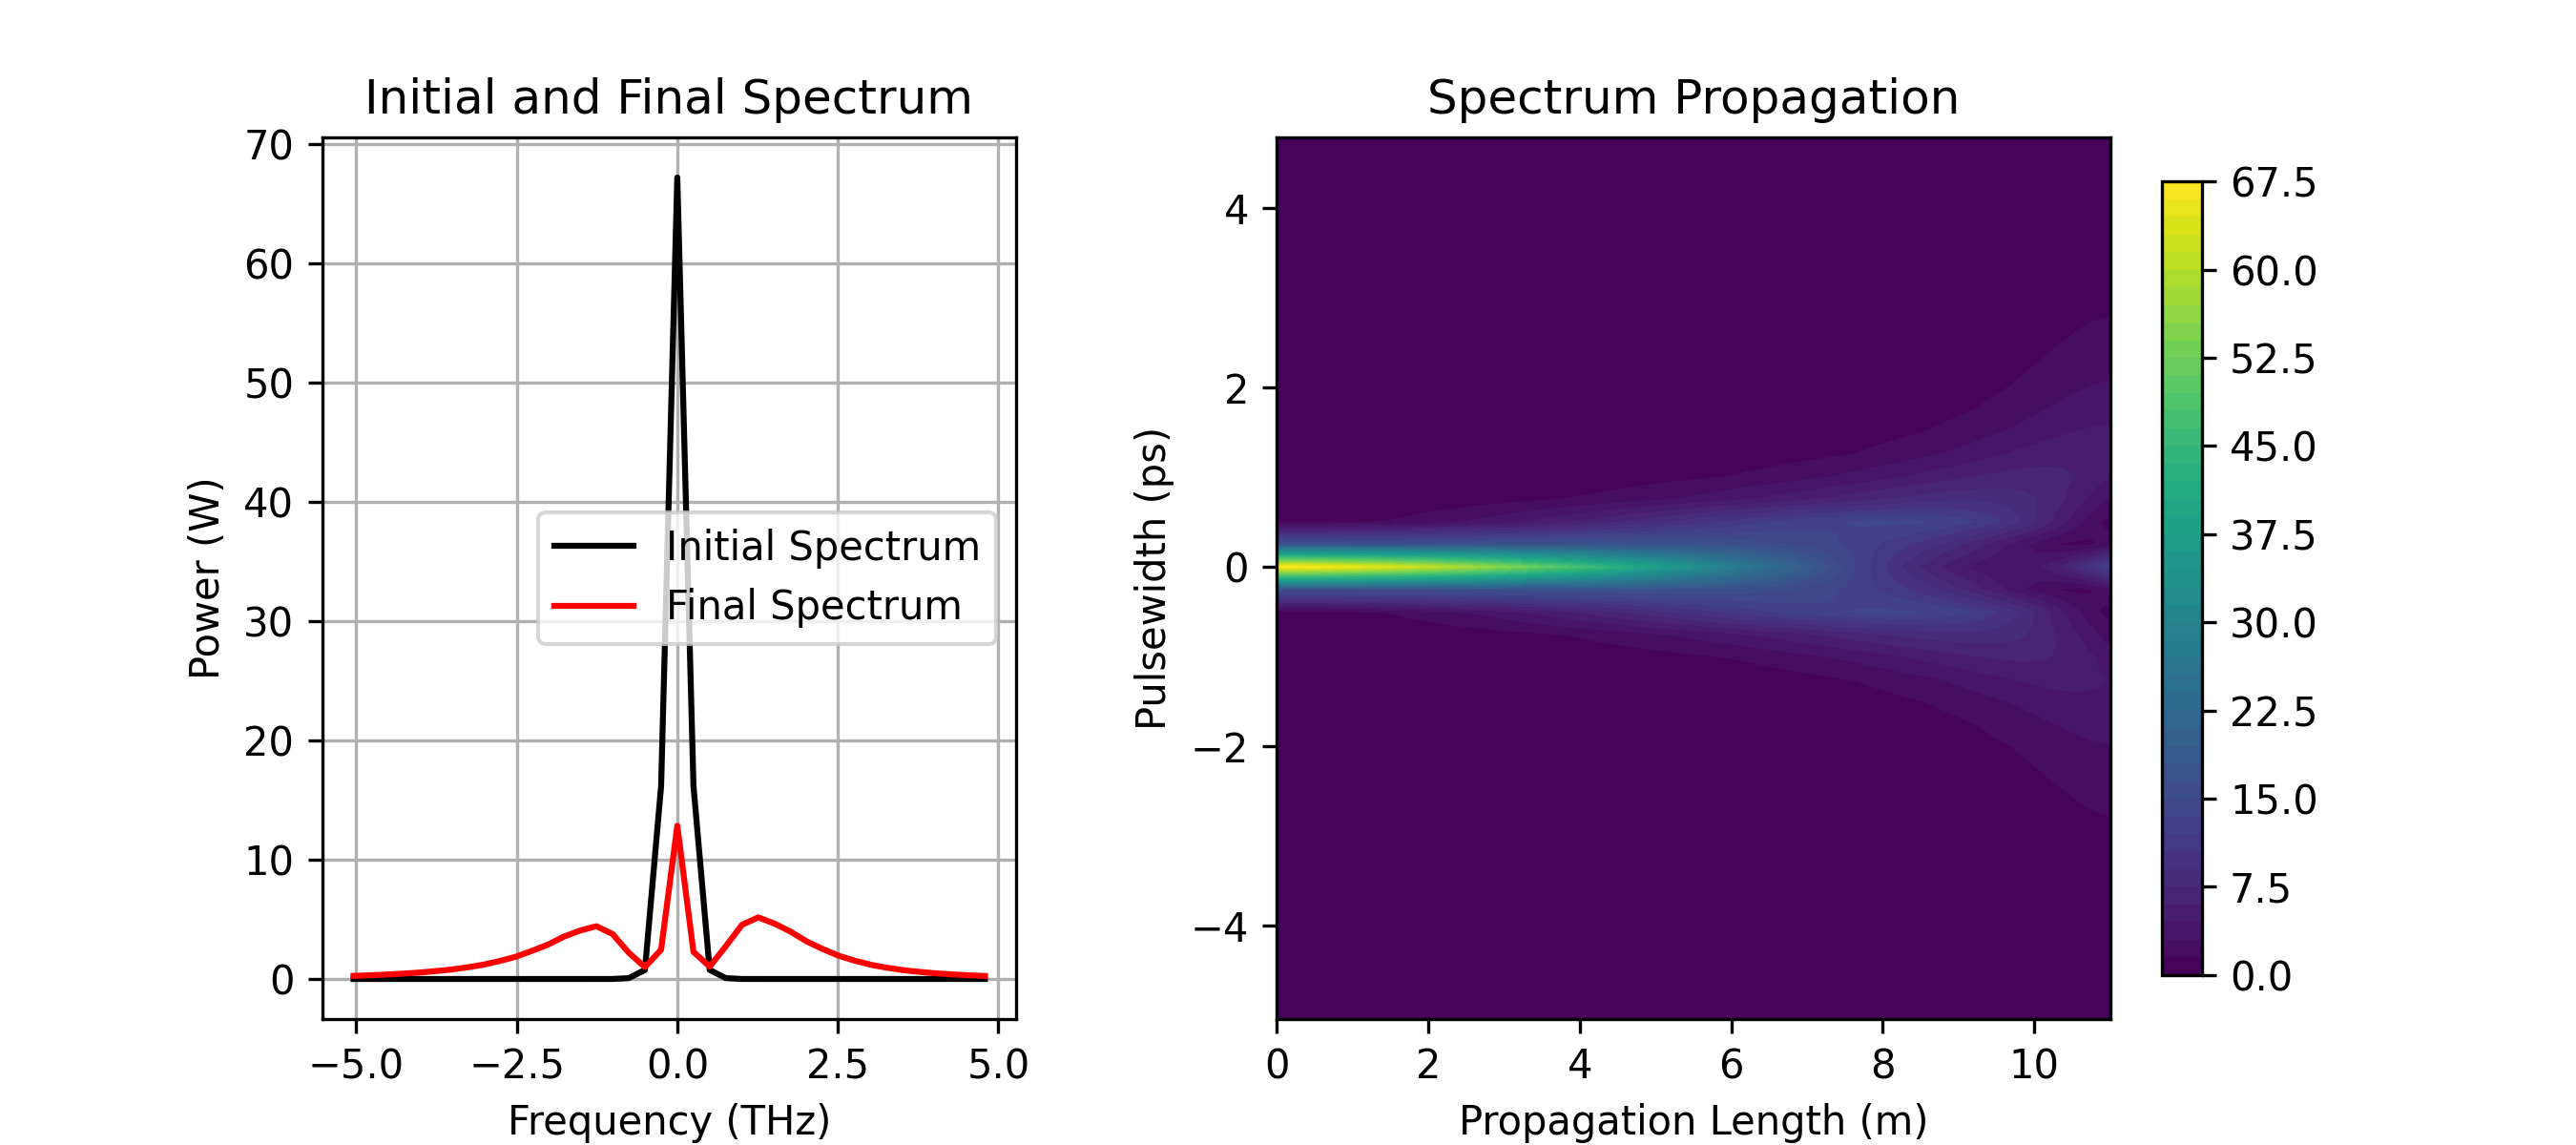
\includegraphics[width=1\linewidth]{Gambar/GroundTruthS3D.png}
    \caption{Spektrum Ground Truth (SSFM)}
    (a) Kondisi Awal dan Akhir; (b) Perambatan Spektrum
    \label{fig:referenceS}
\end{figure}

Distribusi intensitas pulsa pada domain frekuensi ditunjukkan dalam Gambar \ref{fig:referenceS}, di mana pulsa mengalami pelebaran spektrum frekuensi. Hal ini disebabkan oleh modulasi fase tunggal dalam serat optik. Indeks bias nonlinear serat menyebabkan dihasilkannya fase tambahan seiring perambatan pulsa. Frekuensi pulsa kemudian bergeser menjadi lebih tinggi, menghasilkan spektrum yang lebih lebar. Namun, oleh karena gelombang dengan frekuensi lebih tinggi bergerak lebih cepat, komponen gelombang ini menyebabkan durasi pulsa menjadi lebih pendek sehingga pulsa terkompresi.

\section{Evaluasi Hasil Prediksi Vanilla-PINNs}
Hasil inferensi model Vanilla-PINNs menunjukkan karakteristik yang berbeda-beda pada tiap titik kolokasi. Gambar \ref{fig:pulsePINNs} menunjukkan perbandingan antara data pulsa referensi dan data pulsa prediksi model beserta distribusi nilai error dari tiga sampel model. Prediksi PINNs dibandingkan dengan data referensi SSFM, yang ditunjukkan pada \ref{fig:pulsePINNs} (a), melalui \emph{mean square error} (MSE).

\newpage
\begin{figure}[htbp]
    \centering
    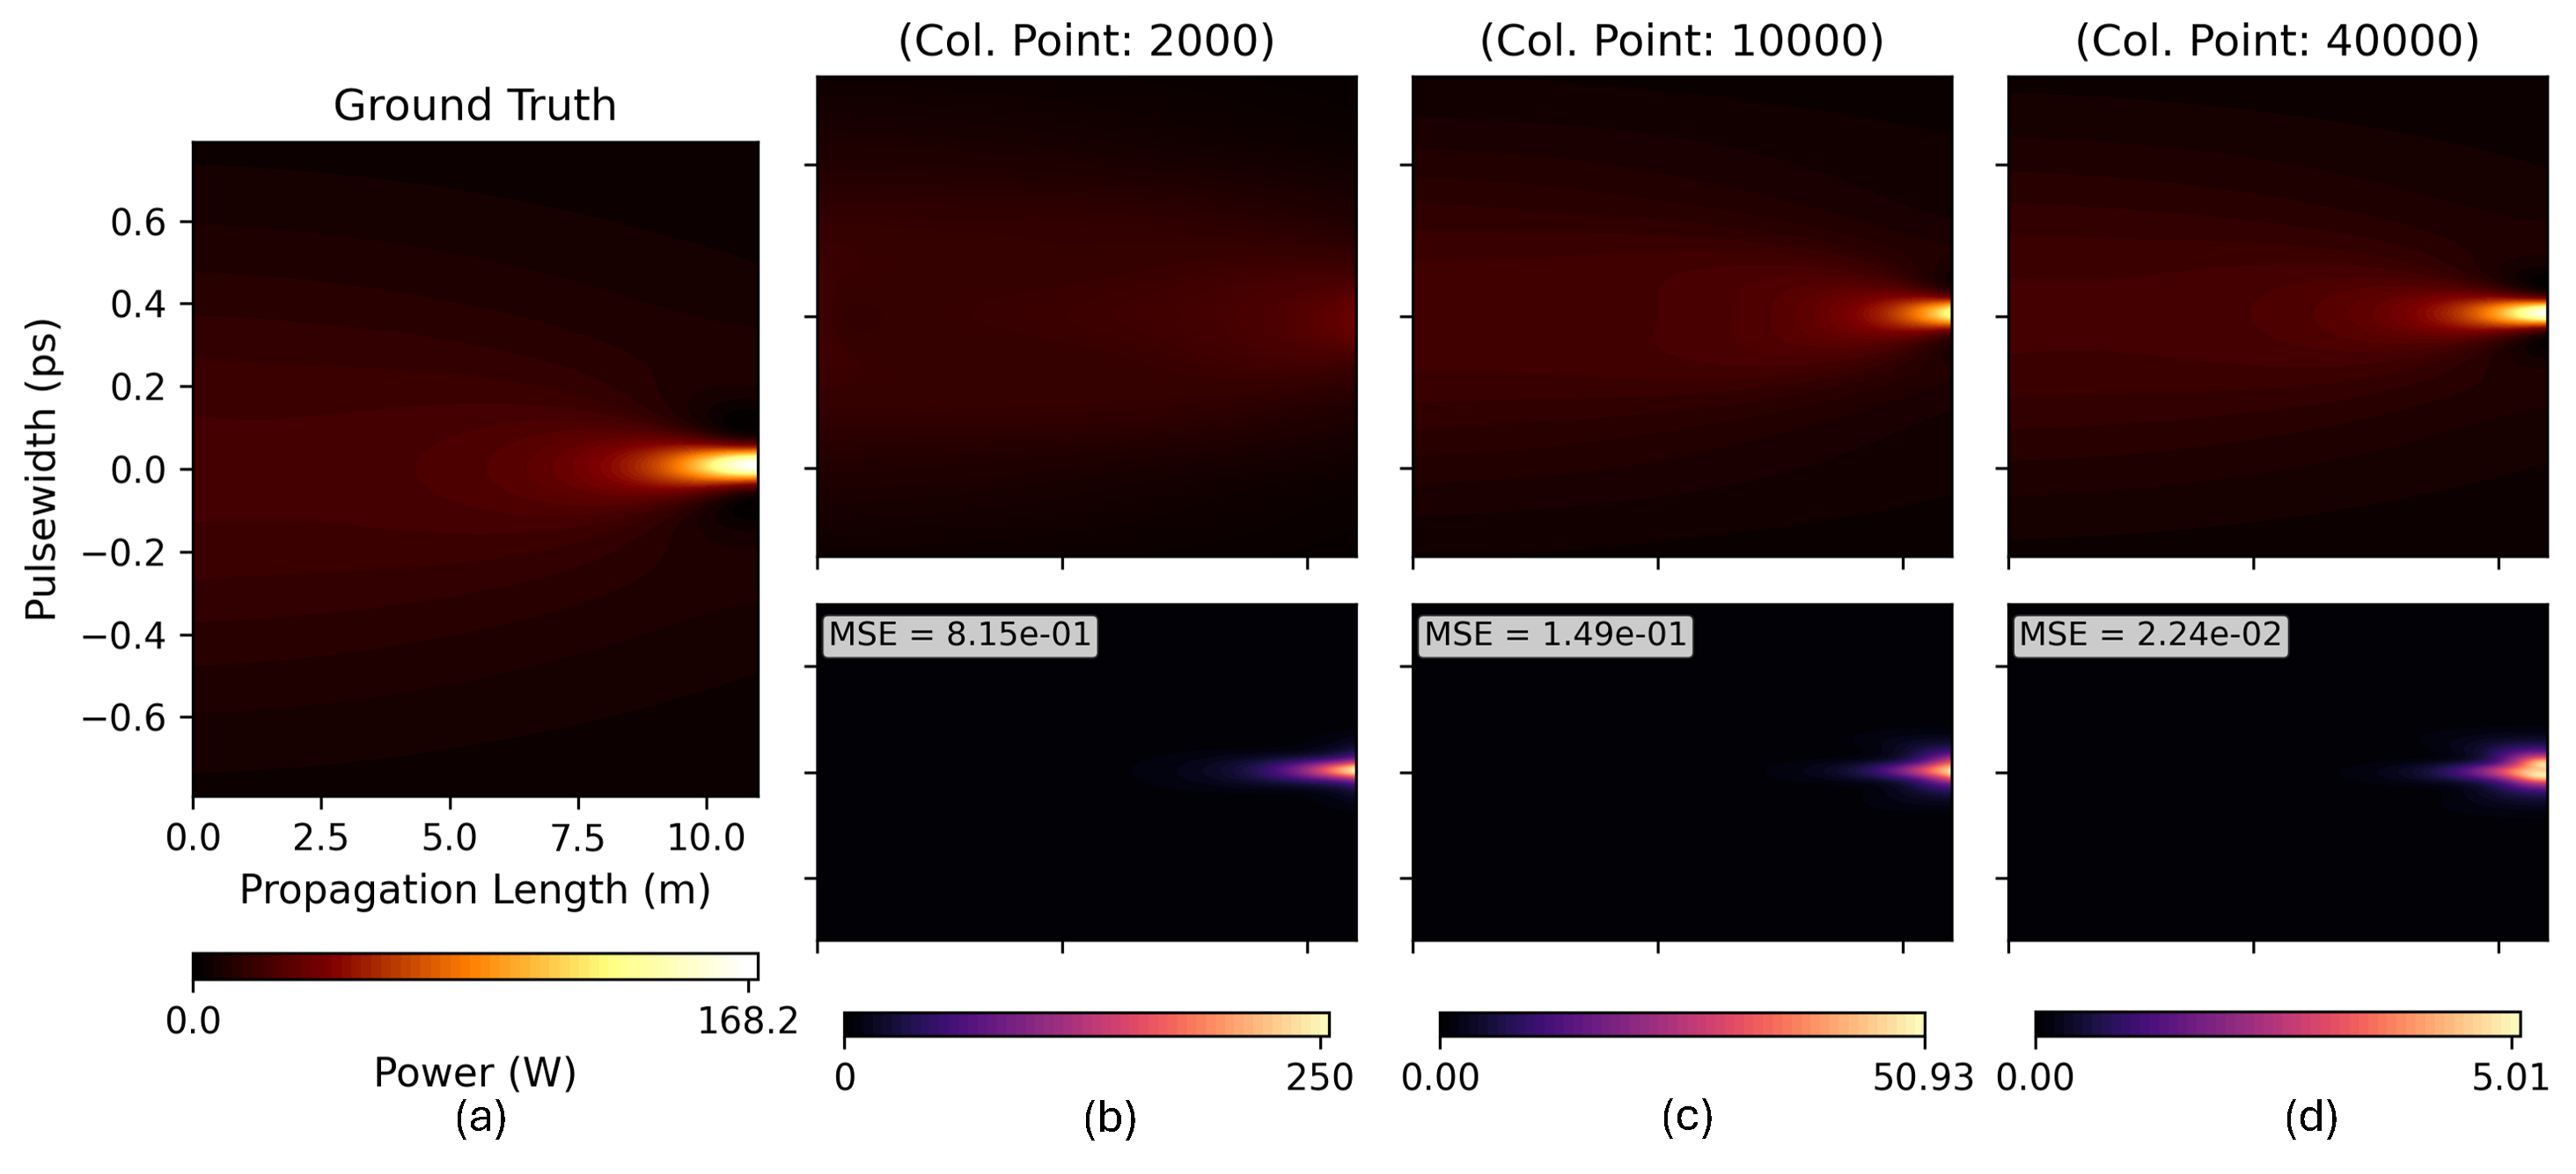
\includegraphics[width=0.9\linewidth]{Gambar/resultsVanilla.png}
    \caption{Distribusi daya pulsa (PINNs)}
    (a) Referensi Numerik, (b)--(d) Prediksi PINNs dengan Titik Kolokasi 2.000, 5.000, dan 10.000 (atas: daya pulsa; bawah: error prediksi (MSE))
    \label{fig:pulsePINNs}
\end{figure}

Ketiga model menunjukkan kesulitan dalam memprediksi proses kompresi pulsa pada jarak 10--11 meter, diberikan pada distribusi error Gambar \ref{fig:pulsePINNs} (b)--(d) bagian bawah. Akan tetapi, ketiga model memiliki nilai MSE yang berbeda. Model dengan 2.000 titik kolokasi tidak mampu menangkap karakteristik penguatan pulsa dengan nilai MSE 0.815. Selain itu, terdapat peningkatan pada model dengan 10.000 titik kolokasi dengan MSE 0.149. Hasil terbaik diperoleh pada model dengan 40.000 titik kolokasi yang mampu dengan baik menangkap proses perambatan pulsa dengan MSE $2.204\times10^{-2}$.

Gambar \ref{fig:specPINNs} menunjukkan bagaimana transformasi prediksi model PINNs pada domain spektral. Kesulitan model dalam memodelkan penguatan pulsa menyebabkan nilai error yang terfokus pada proses pelebaran spektrum pada jarak 10--11 meter. Sama halnya dengan Gambar \ref{fig:pulsePINNs}, dibandingkan dengan referensi numerik pada \ref{fig:specPINNs} (a), model dengan 2.000 sampel domain tidak mampu menangkap pergeseran spektrum dengan benar, sementara hasil terbaik turut diperoleh pada model dengan 40.000 sampel. Akan tetapi, nilai MSE domain spektral memberikan hasil yang lebih kecil dari domain temporal. Hal ini dapat dijelaskan dengan nilai daya spektrum yang lebih kecil dan tersebar dibanding daya pulsa yang lebih besar dan terfokus pada titik kompresi. Oleh karena itu, akumulasi error dari daya temporal lebih besar dari daya spektrum.

\begin{figure}[htbp]
    \centering
    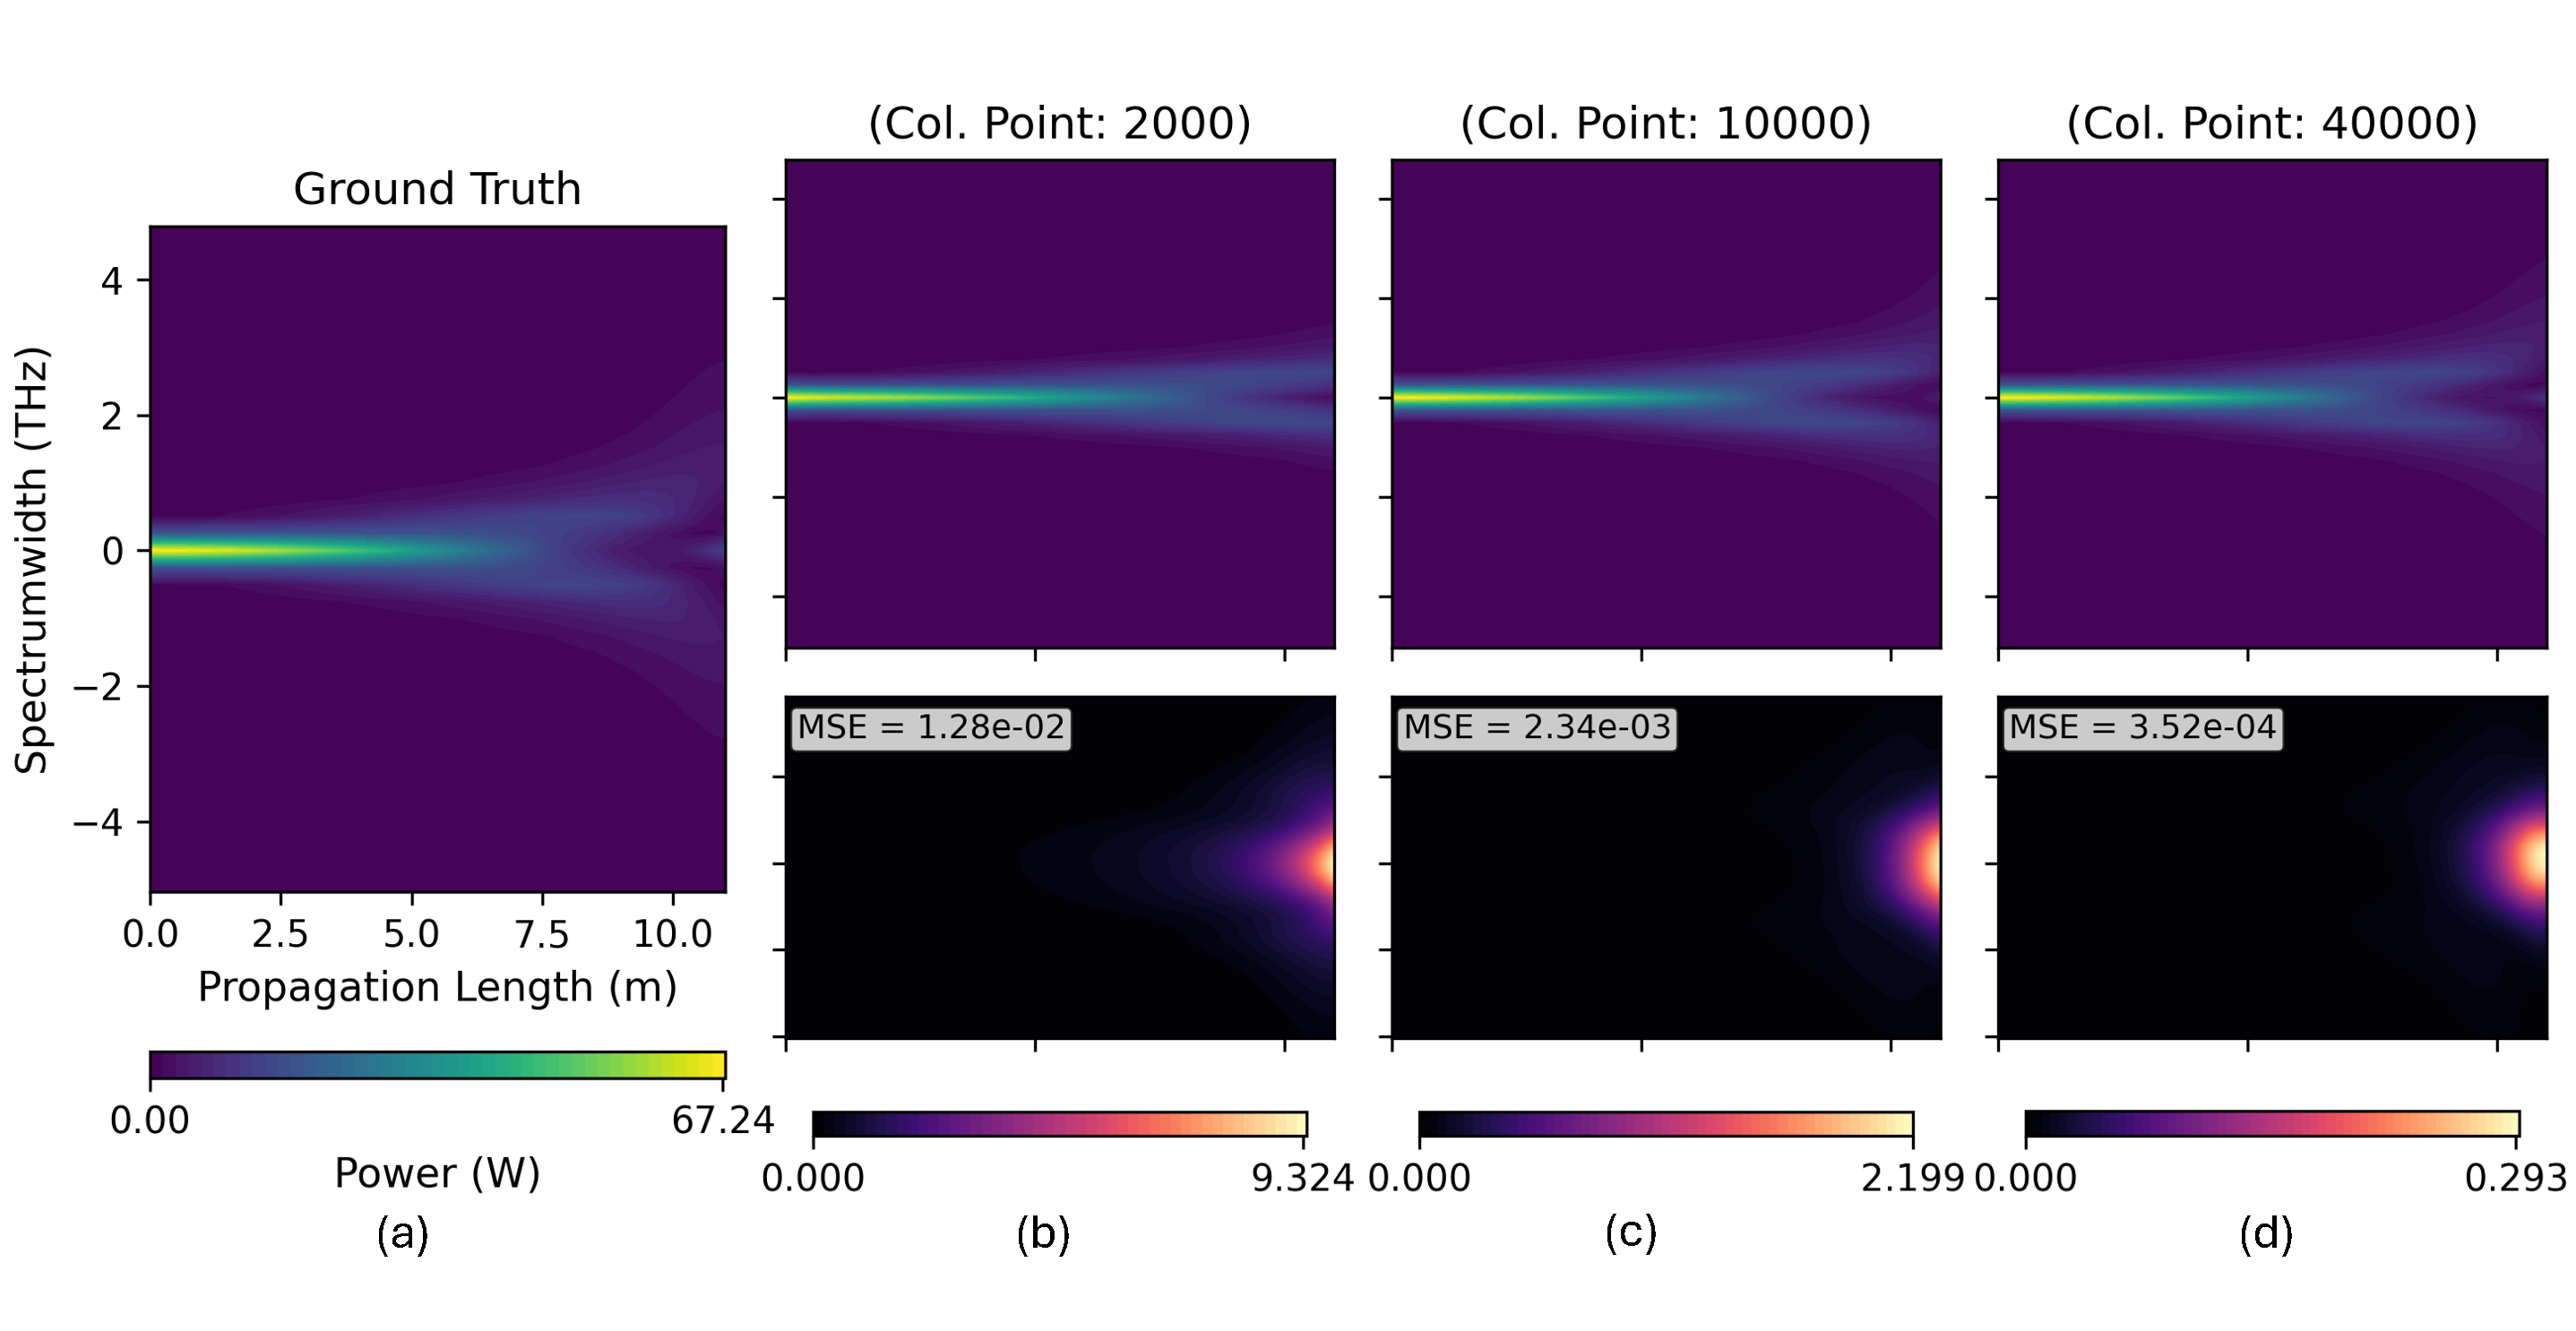
\includegraphics[width=0.9 \linewidth]{Gambar/resultsVanillaS.png}
    \caption{Distribusi daya spektrum (PINNs)}
    (a) Referensi numerik, (b)–(d) Prediksi PINNs dengan Titik Kolokasi 2.000, 5.000, dan 10.000 (atas: daya spektrum; bawah: error prediksi (MSE))
    \label{fig:specPINNs}
\end{figure}

Informasi dari seluruh nilai MSE dari percobaan Vanilla-PINNs terdapat pada Gambar \ref{fig:VPINN-MSE}. Nilai MSE memberikan distribusi yang lebar pada jumlah titik kolokasi 2.000 dan 5.000. Inferensi PINNs dapat menghasilkan prediksi yang baik atau buruk berdasarkan titik kolokasi tersebar. Pada persebaran titik kolokasi yang renggang, model sangat sensitif terhadap bagaimana sampel domain dipilih. Hal ini menyebabkan hasil yang tidak konsisten ketika ketika diujicobakan pada pembelajaran dengan \emph{random seed} yang berbeda.

\newpage

\begin{figure}[htbp]
    \centering
    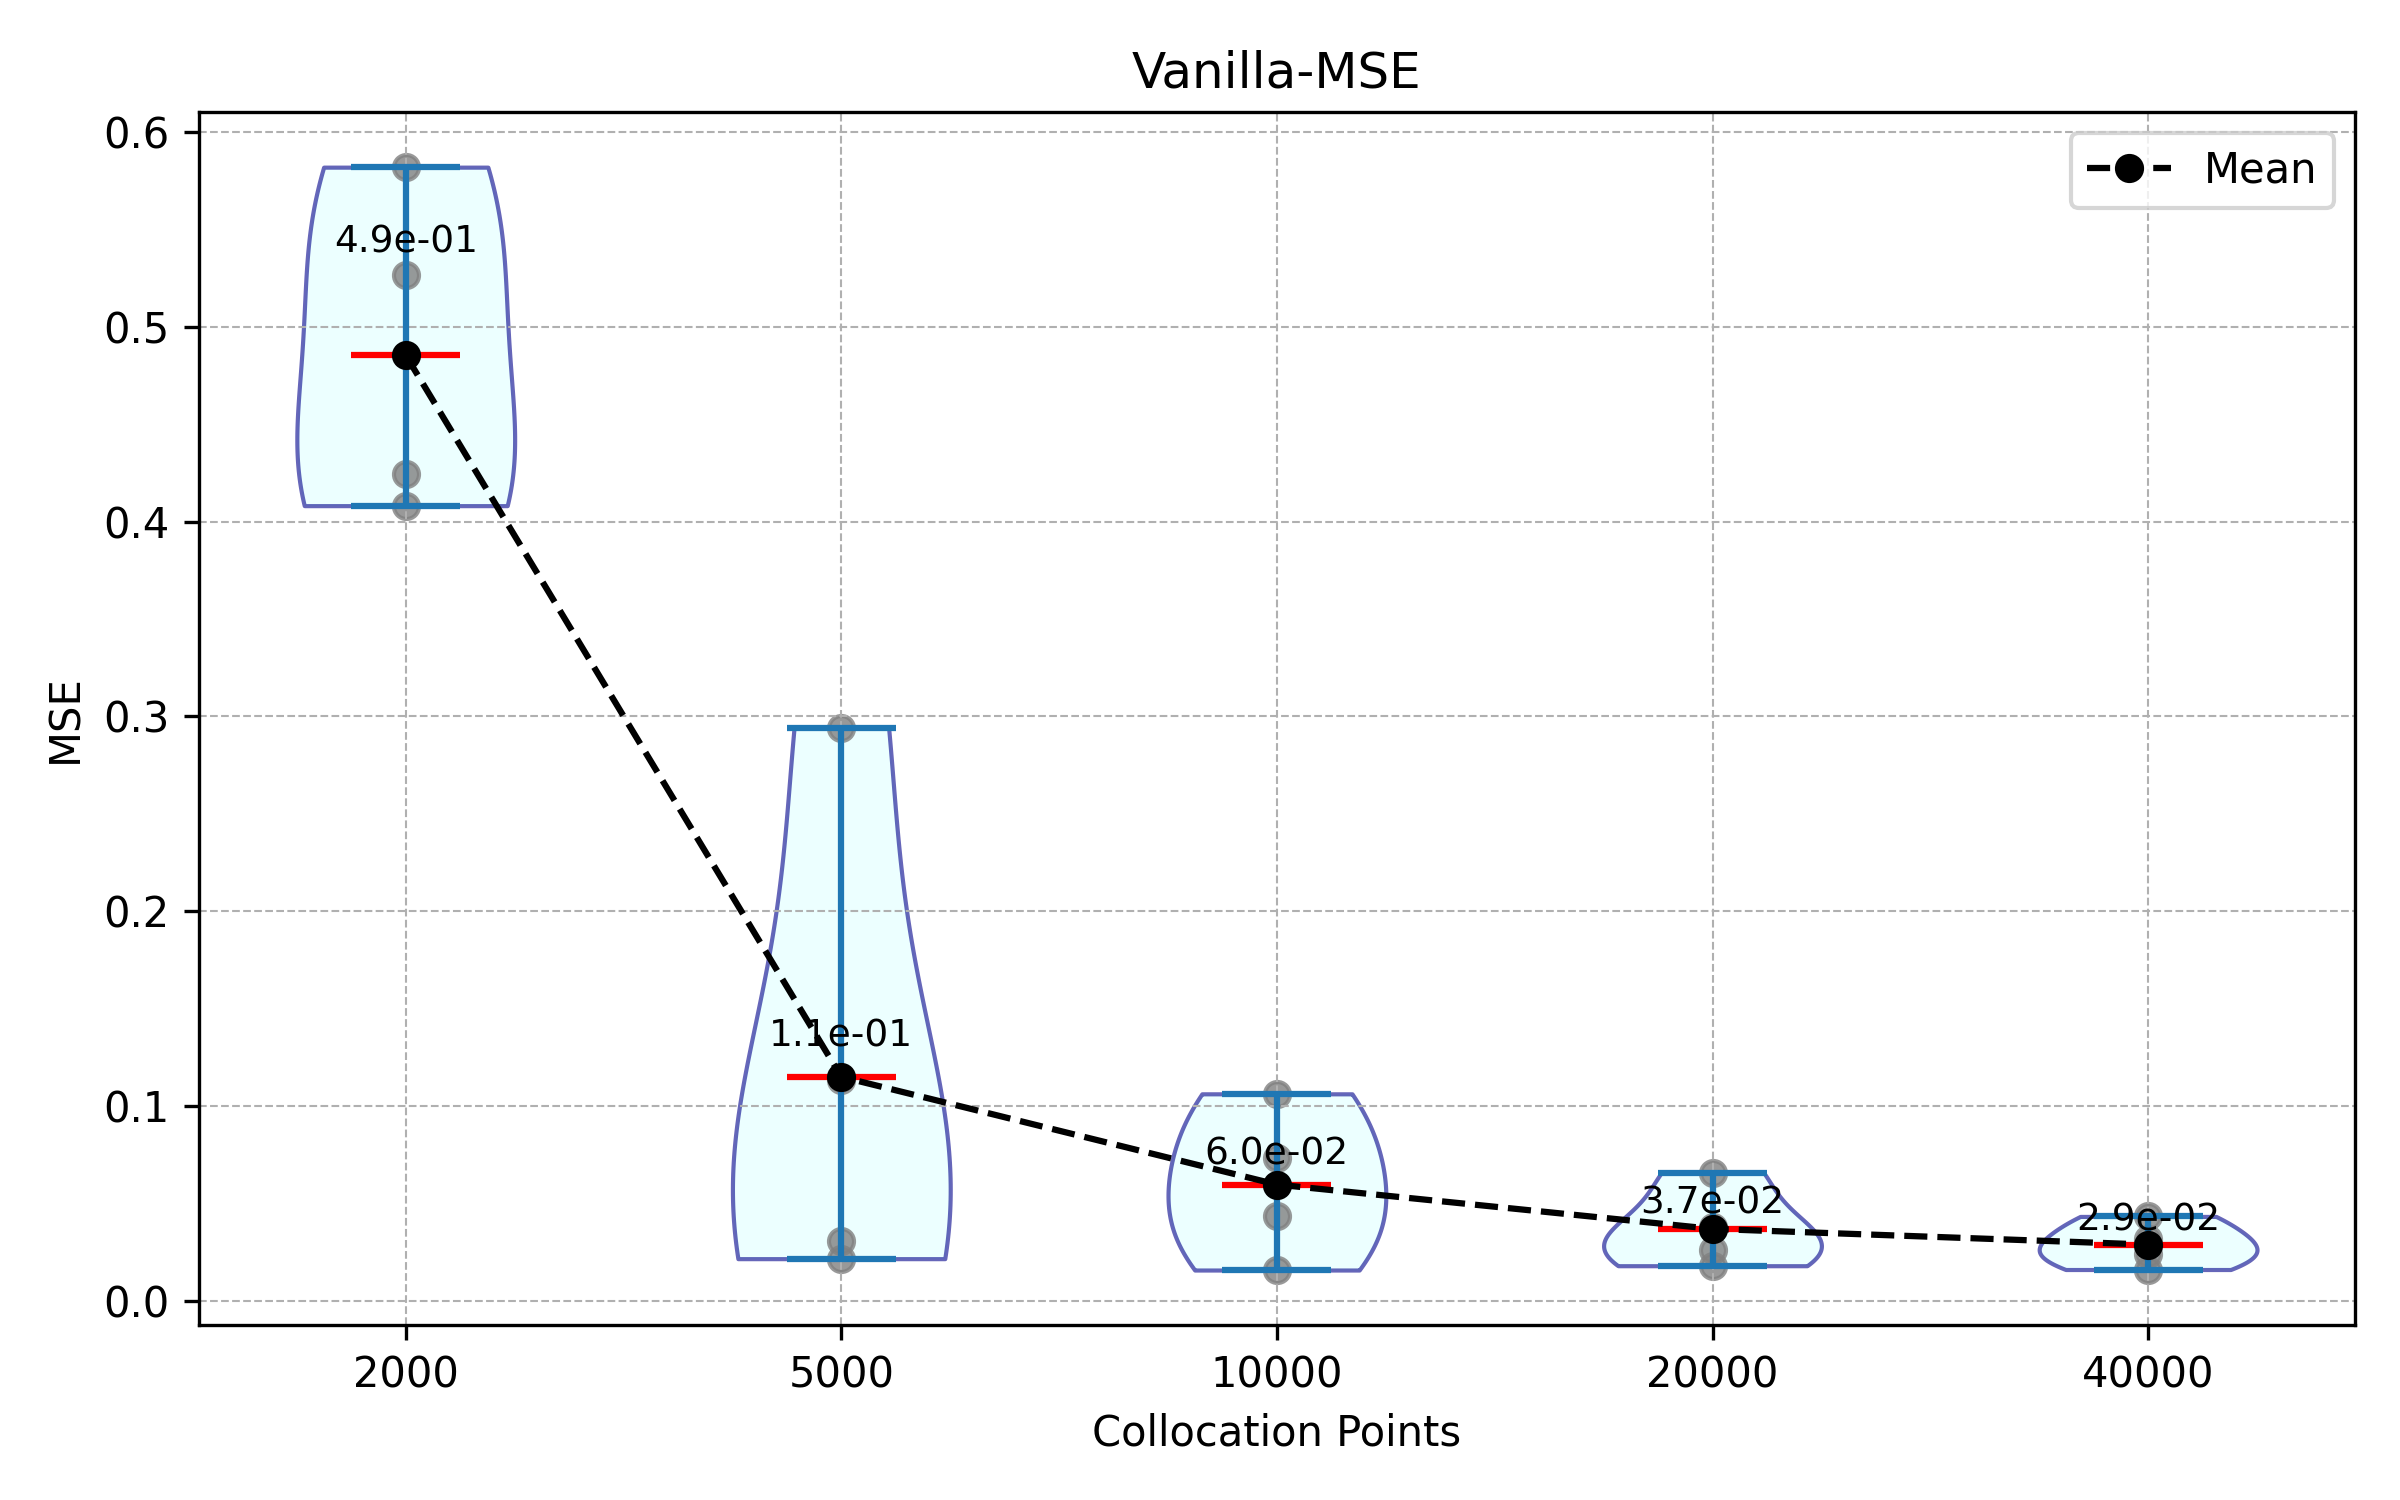
\includegraphics[width=0.9 \linewidth]{Gambar/colPoints-Error.png}
    \caption{Nilai MSE Prediksi Temporal PINNs}
    \label{fig:VPINN-MSE}
\end{figure} 

Sebaliknya, jumlah titik kolokasi yang lebih besar memberikan hasil yang lebih konsisten dengan persebaran nilai MSE yang lebih sempit. Distribusi titik yang menjadi lebih rapat menyebabkan model mendapatkan informasi yang cukup selama pembelajaran. Oleh sebab itu, model dengan 40.000 sampel memiliki tingkat presisi terbaik dari jumlah sampel yang lain. 

Akurasi model dapat diamati melalui rata-rata nilai MSE dalam keempat perulangan. Sebuah garis pada gambar \ref{fig:VPINN-MSE} ditarik terhadap nilai rata-rata MSE pada setiap jumlah kolokasi. Garis tersebut menunjukkan penurunan rata-rata MSE secara eksponensial seiring dengan meningkatnya jumlah sampel. Dapat disimpulkan bahwa konvergensi nilai MSE menunjukkan peningkatan akurasi dan presisi seiring dengan bertambahnya jumlah kolokasi.

Akan tetapi, meningkatkan jumlah sampel kolokasi berpotensi meningkatkan waktu pembelajaran dan kompleksitas komputasi secara signifikan. Hal ini disebabkan oleh bertambahnya jumlah perhitungan residual yang perlu dilakukan model PINNs pada setiap iterasi. Oleh karena itu, pemilihan jumlah titik kolokasi yang optimal menjadi krusial untuk mencapai keseimbangan antara akurasi prediksi dan efisiensi pelatihan.

Proses pembelajaran PINNs dilakukan menggunakan strategi optimasi ADAM dilanjutkan dengan strategi L-BFGS. Optimasi ADAM mengakumulasi gradien dan variansi gradien dari proses optimasi sebelumnya sebagai fungsi momentum. Strategi optimasi ini mampu menyesuaikan proses pembelajaran secara dinamis dan memberikan optimasi yang lebih terarah. Akan tetapi, fungsi biaya residual $\mathcal{H}$ yang melibatkan turunan hingga derajat ketiga menyebabkan gradien numerik dari proses optimasi yang tidak stabil. Hal ini menyebabkan terjadinya fluktuasi yang signifikan pada optimasi ADAM selama 40.000 epoch.

\begin{figure}[htbp]
    \centering
    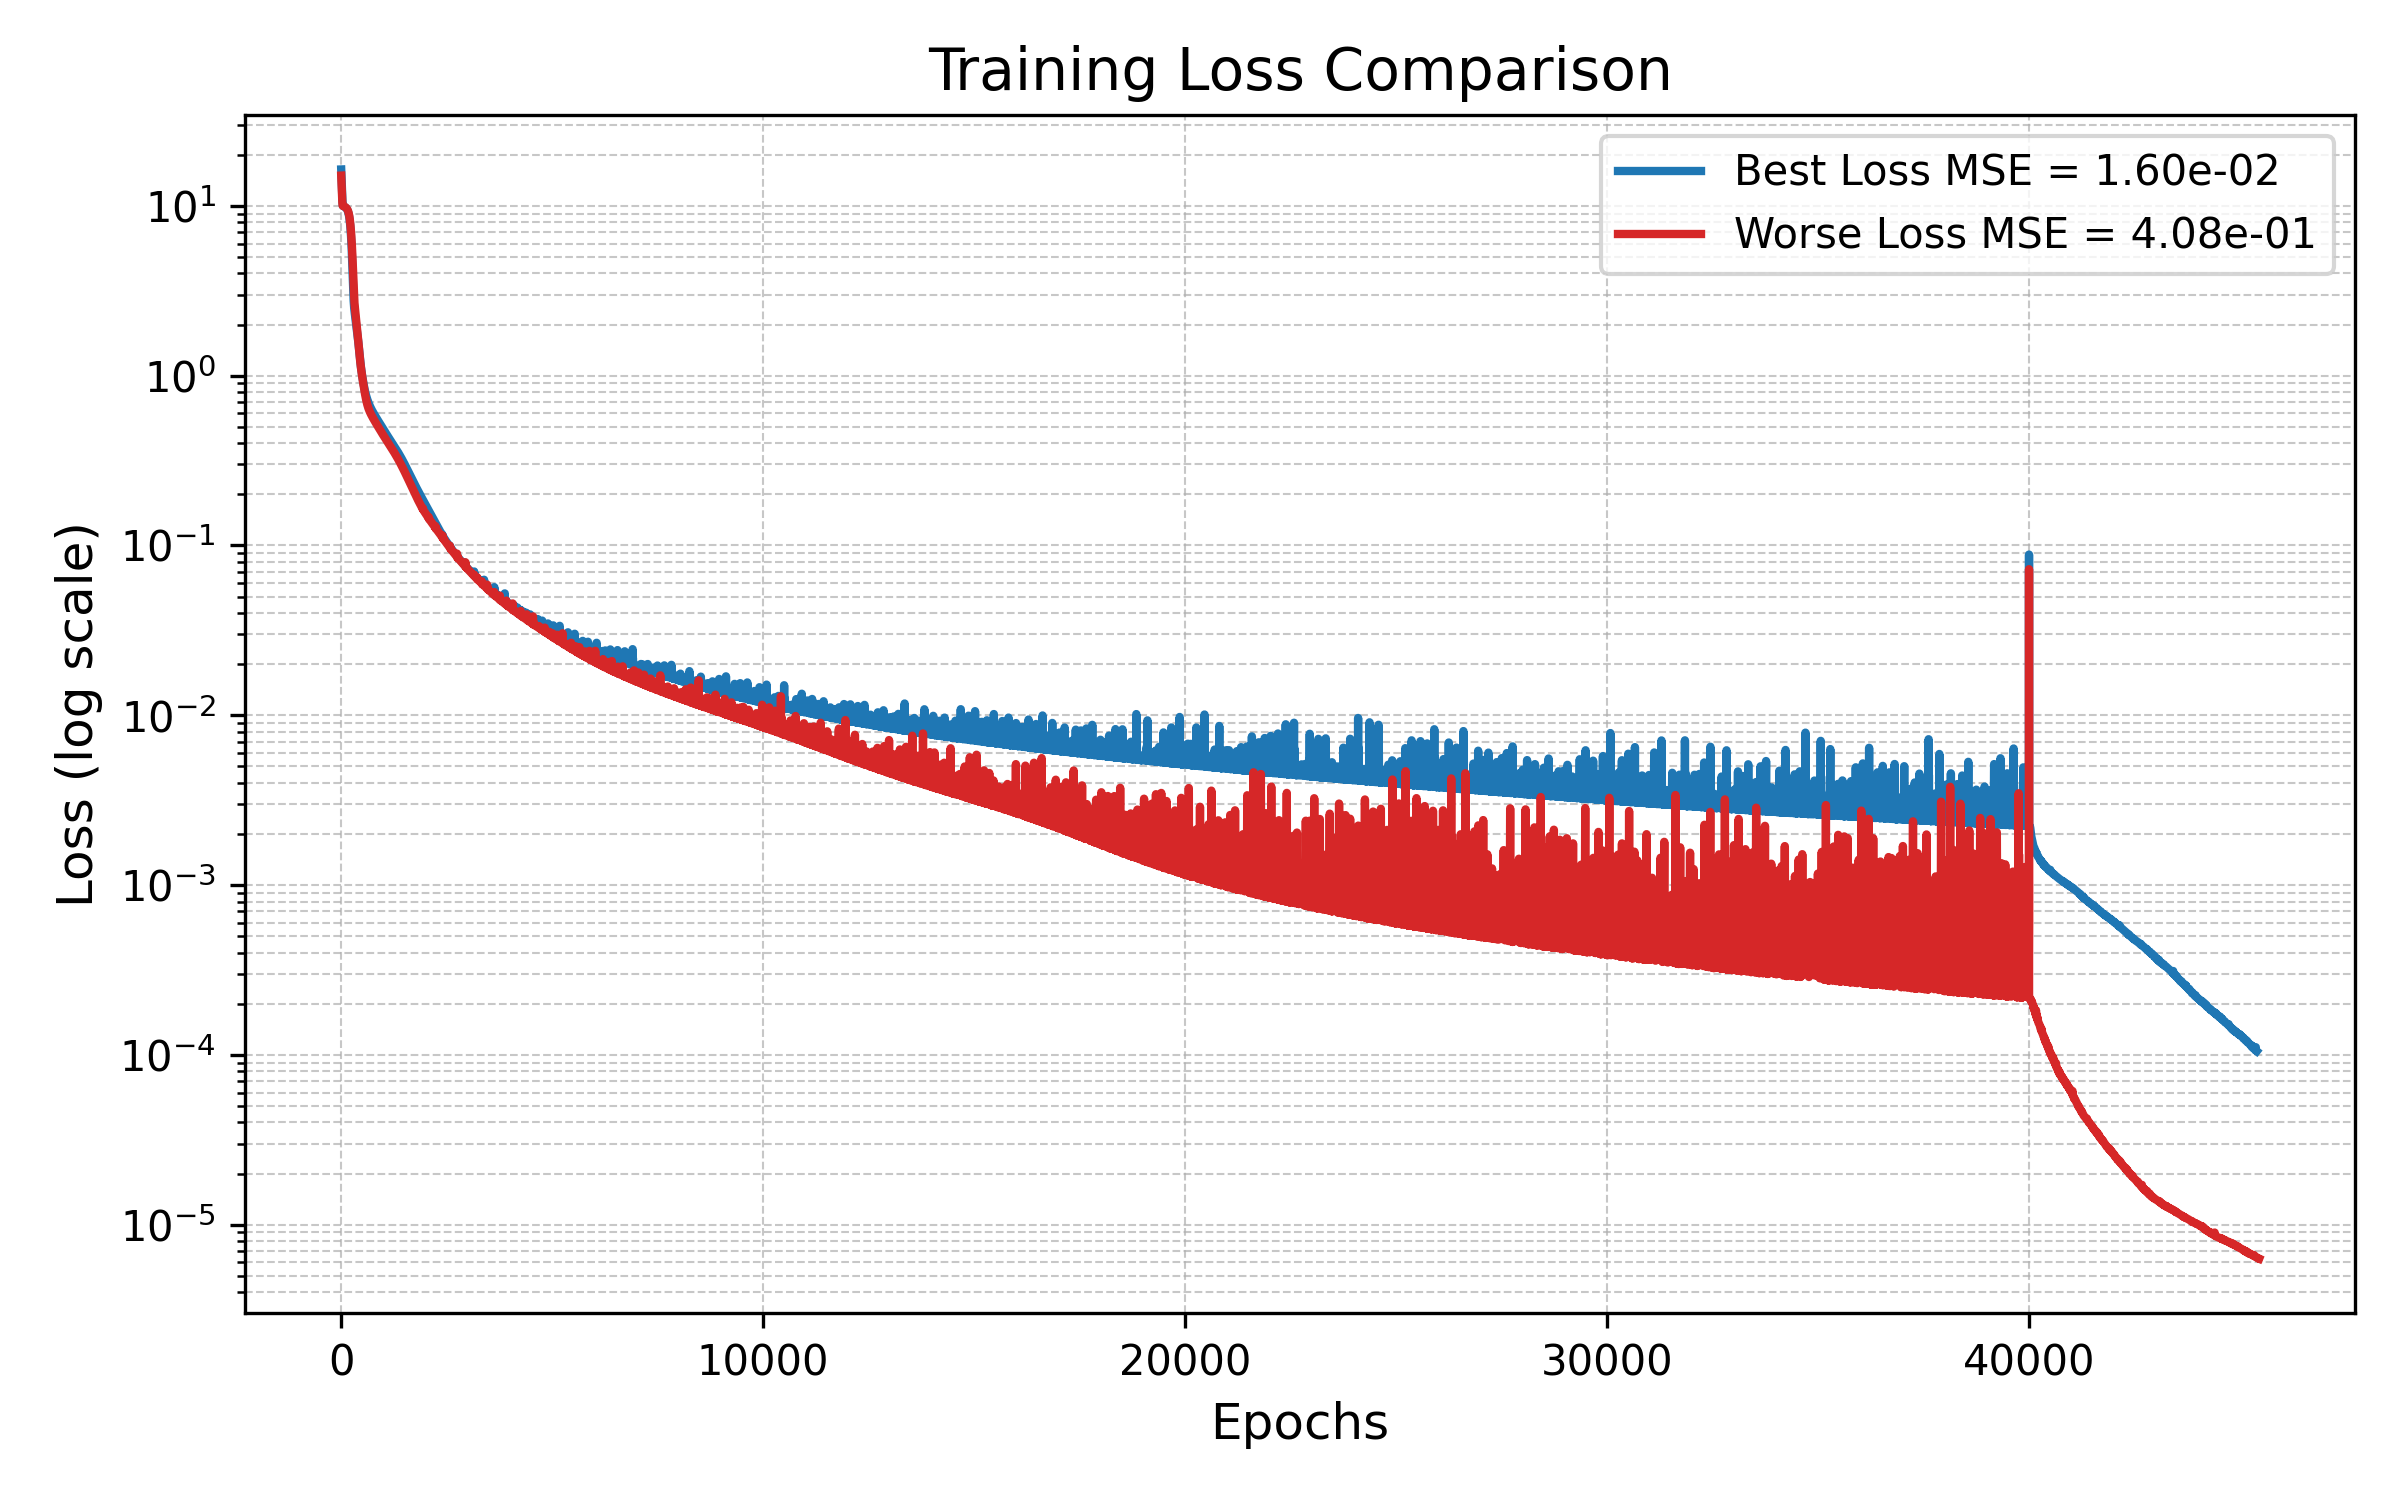
\includegraphics[width=0.9 \linewidth]{Gambar/Loss-Comparison.png}
    \caption{Grafik Fungsi Loss Vanilla-PINNs}
    \label{fig:loss-PINNs}
\end{figure}

Setelah fase awal ADAM, pelatihan dilanjutkan menggunakan algoritma L-BFGS yang bersifat deterministik dan memanfaatkan informasi kurva loss secara global. L-BFGS berperan sebagai metode penyelaman yang secara tajam dan efisien mengarahkan model menuju solusi optimal. Proses penyelaman terlihat dari penurunan \emph{residual loss} yang sangat cepat pada 5.000 epoch terakhir. Namun, L-BFGS memerlukan penggunaan dan penyimpanan matriks Hessian aproksimasi dalam jumlah besar sehingga jumlah epoch perlu dibatasi untuk menjaga efisiensi waktu pelatihan.

Nilai loss pada Gambar \ref{fig:loss-PINNs} menunjukkan bahwa model dengan 2.000 titik collocation memiliki performa konvergensi \emph{residual loss} yang tampak lebih kecil dibandingkan model dengan 40.000 titik. Namun, nilai MSE antara kedua model justru menunjukkan hasil yang bertolak belakang. Seperti yang telah disimpulkan, model dengan jumlah titik kolokasi yang lebih banyak selama pembelajaran memberikan prediksi yang lebih akurat. 

Kontradiksi tersebut dapat dijelaskan dengan fenomena \emph{underfitting} pada model dengan jumlah titik kolokasi yang terlalu sedikit. Dikarenakan cakupan ruang solusi yang terbatas, model dapat dengan mudah menyesuaikan diri pada titik tersebut tanpa benar-benar memahami perilaku fisis dari solusi sebenarnya. Akibatnya, meskipun \emph{residual loss}—yang dihitung hanya pada titik-titik tersebut terlihat kecil, model gagal melakukan generalisasi dengan baik, yang tercermin pada nilai MSE yang tinggi ketika diuji terhadap solusi sebenarnya.

\section {Evaluasi Hasil Prediksi SAS-PINNs}
SMOTE merupakan salah satu teknik \emph{oversampling} yang digunakan untuk menyeimbangkan distribusi data minoritas dengan data mayoritas dalam proses klasifikasi. Akan tetapi, pada strategi SAS-PINNs, SMOTE digunakan untuk memfokuskan titik kolokasi tambahan pada area dengan kesulitan konvergensi tinggi. Kedua parameter SAS-PINNs memiliki peranan masing-masing. Nilai Ambang menyatakan luas area penambahan data di mana semakin kecil nilainya, \emph{oversampling} akan dilakukan pada area dengan residual tertinggi secara lebih terfokus. Rasio \emph{Oversampling} menyatakan seberapa banyak data yang akan ditambahkan melalui perbandingan dari target data minoritas terhadap data mayoritas.

Secara konvensional, SMOTE digunakan untuk menyeimbangkan jumlah data minoritas terhadap data mayoritas. Hal ini dilakukan dengan mengatur rasio \emph{oversampling} sebagai satu yang menghasilkan perbandingan jumlah data minoritas dan mayoritas menjadi 1:1. Akan tetapi, SAS-PINNs memiliki paradigma yang berbeda di mana SMOTE tidak digunakan untuk menyeimbangkan titik kolokasi. Gambar \ref{fig:Bad-SAS-PINNs} menunjukkan apa yang terjadi pada inferensi model jika jumlah rasio \emph{oversampling} diatur sebagai 1 untuk tiap nilai ambang pada titik kolokasi 10.000.


\begin{figure}[htbp]
    \centering
    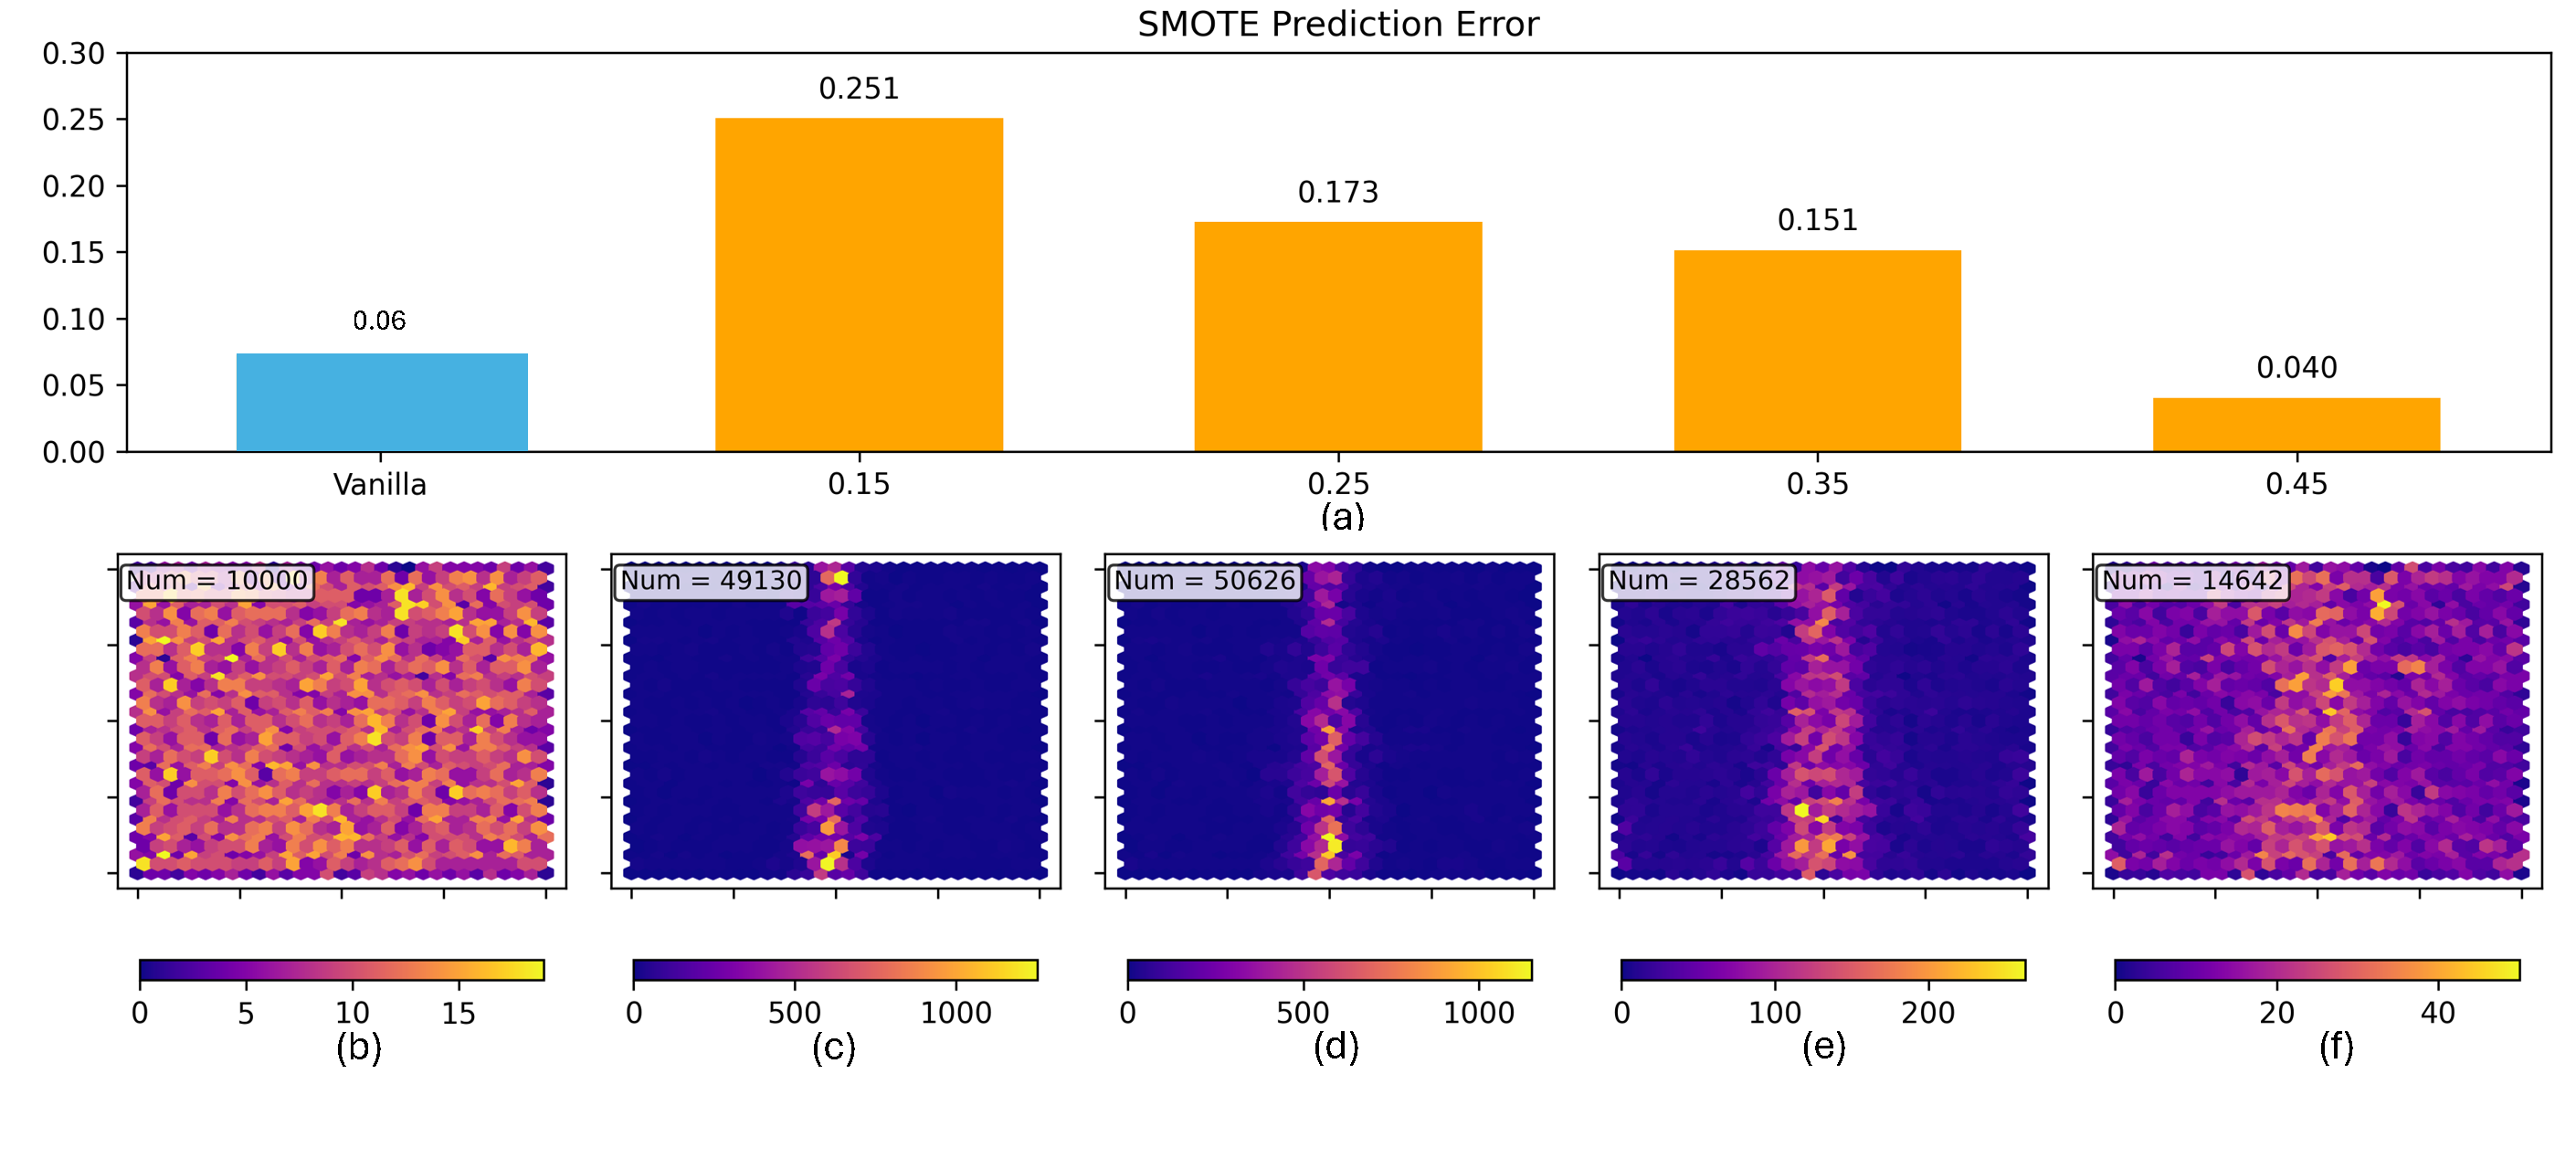
\includegraphics[width=0.9 \linewidth]{Gambar/smoteDistribution.png}
    \caption{Nilai MSE SAS-PINNs dengan Rasio 1}
    (a) Rata-Rata MSE Vanilla-PINNs dan MSE SAS-PINNs untuk Empat Perlakuan Nilai Ambang; (b) Distribusi Sampel Vanilla-PINNs; (c)-(f) Distribusi Sampel SAS-PINNs pada Nilai Ambang 0.15, 0.25, 0.35, 0.45
    \label{fig:Bad-SAS-PINNs}
\end{figure}

Dengan mengatur nilai rasio sebagai 1, jumlah titik kolokasi yang ditambahkan menjadi tidak terkontrol pada nilai ambang yang kecil. Sebagai contoh, pada nilai ambang 0.15, sebanyak 39.130 titik ditambahkan pada area dengan residual tertinggi. Hal ini justru merusak distribusi data secara signifikan, di mana mula-mula model hanya memiliki 10.000 titik kolokasi yang tersebar seragam. Rusaknya distribusi data mengakibatkan model tidak dapat melakukan konvergensi pada keseluruhan domain secara menyeluruh, menyebabkan peningkatan nilai MSE yang mencapai 0.251.

Akan tetapi, permasalahan ini tidak ditunjukkan pada nilai ambang 0.45, di mana hanya 4.642 data yang ditambahkan ke dalam model. Penambahan data ini terbukti menurunkan nilai MSE menjadi 0.04. Oleh karena itu, pengaturan rasio \emph{oversampling} perlu mempertimbangkan nilai ambang yang digunakan, di mana semakin kecil nilai ambang, perlu digunakan angka rasio yang lebih kecil. Informasi ini menjadi alasan atas digunakannya konfigurasi nilai ambang dan rasio sebagai berikut:

\begin{table}[htbp]
    \centering
    \begin{threeparttable}
        \caption{Nilai Ambang dan Rasio SAS-PINNs}
        \begin{tabular}{|p{5cm}|p{4cm}|}
				\hline
				Nilai Ambang & Rasio \\
                \hline 
                0.45 & 1\\
                \hline
                0.35 & 0.7 \\
                \hline
                0.25 & 0.4 \\
                \hline
                0.15 & 0.25 \\
                \hline
			\end{tabular}
        \label{SAS-config}
    \end{threeparttable}
\end{table} 

\begin{figure}[htbp]
    \centering
    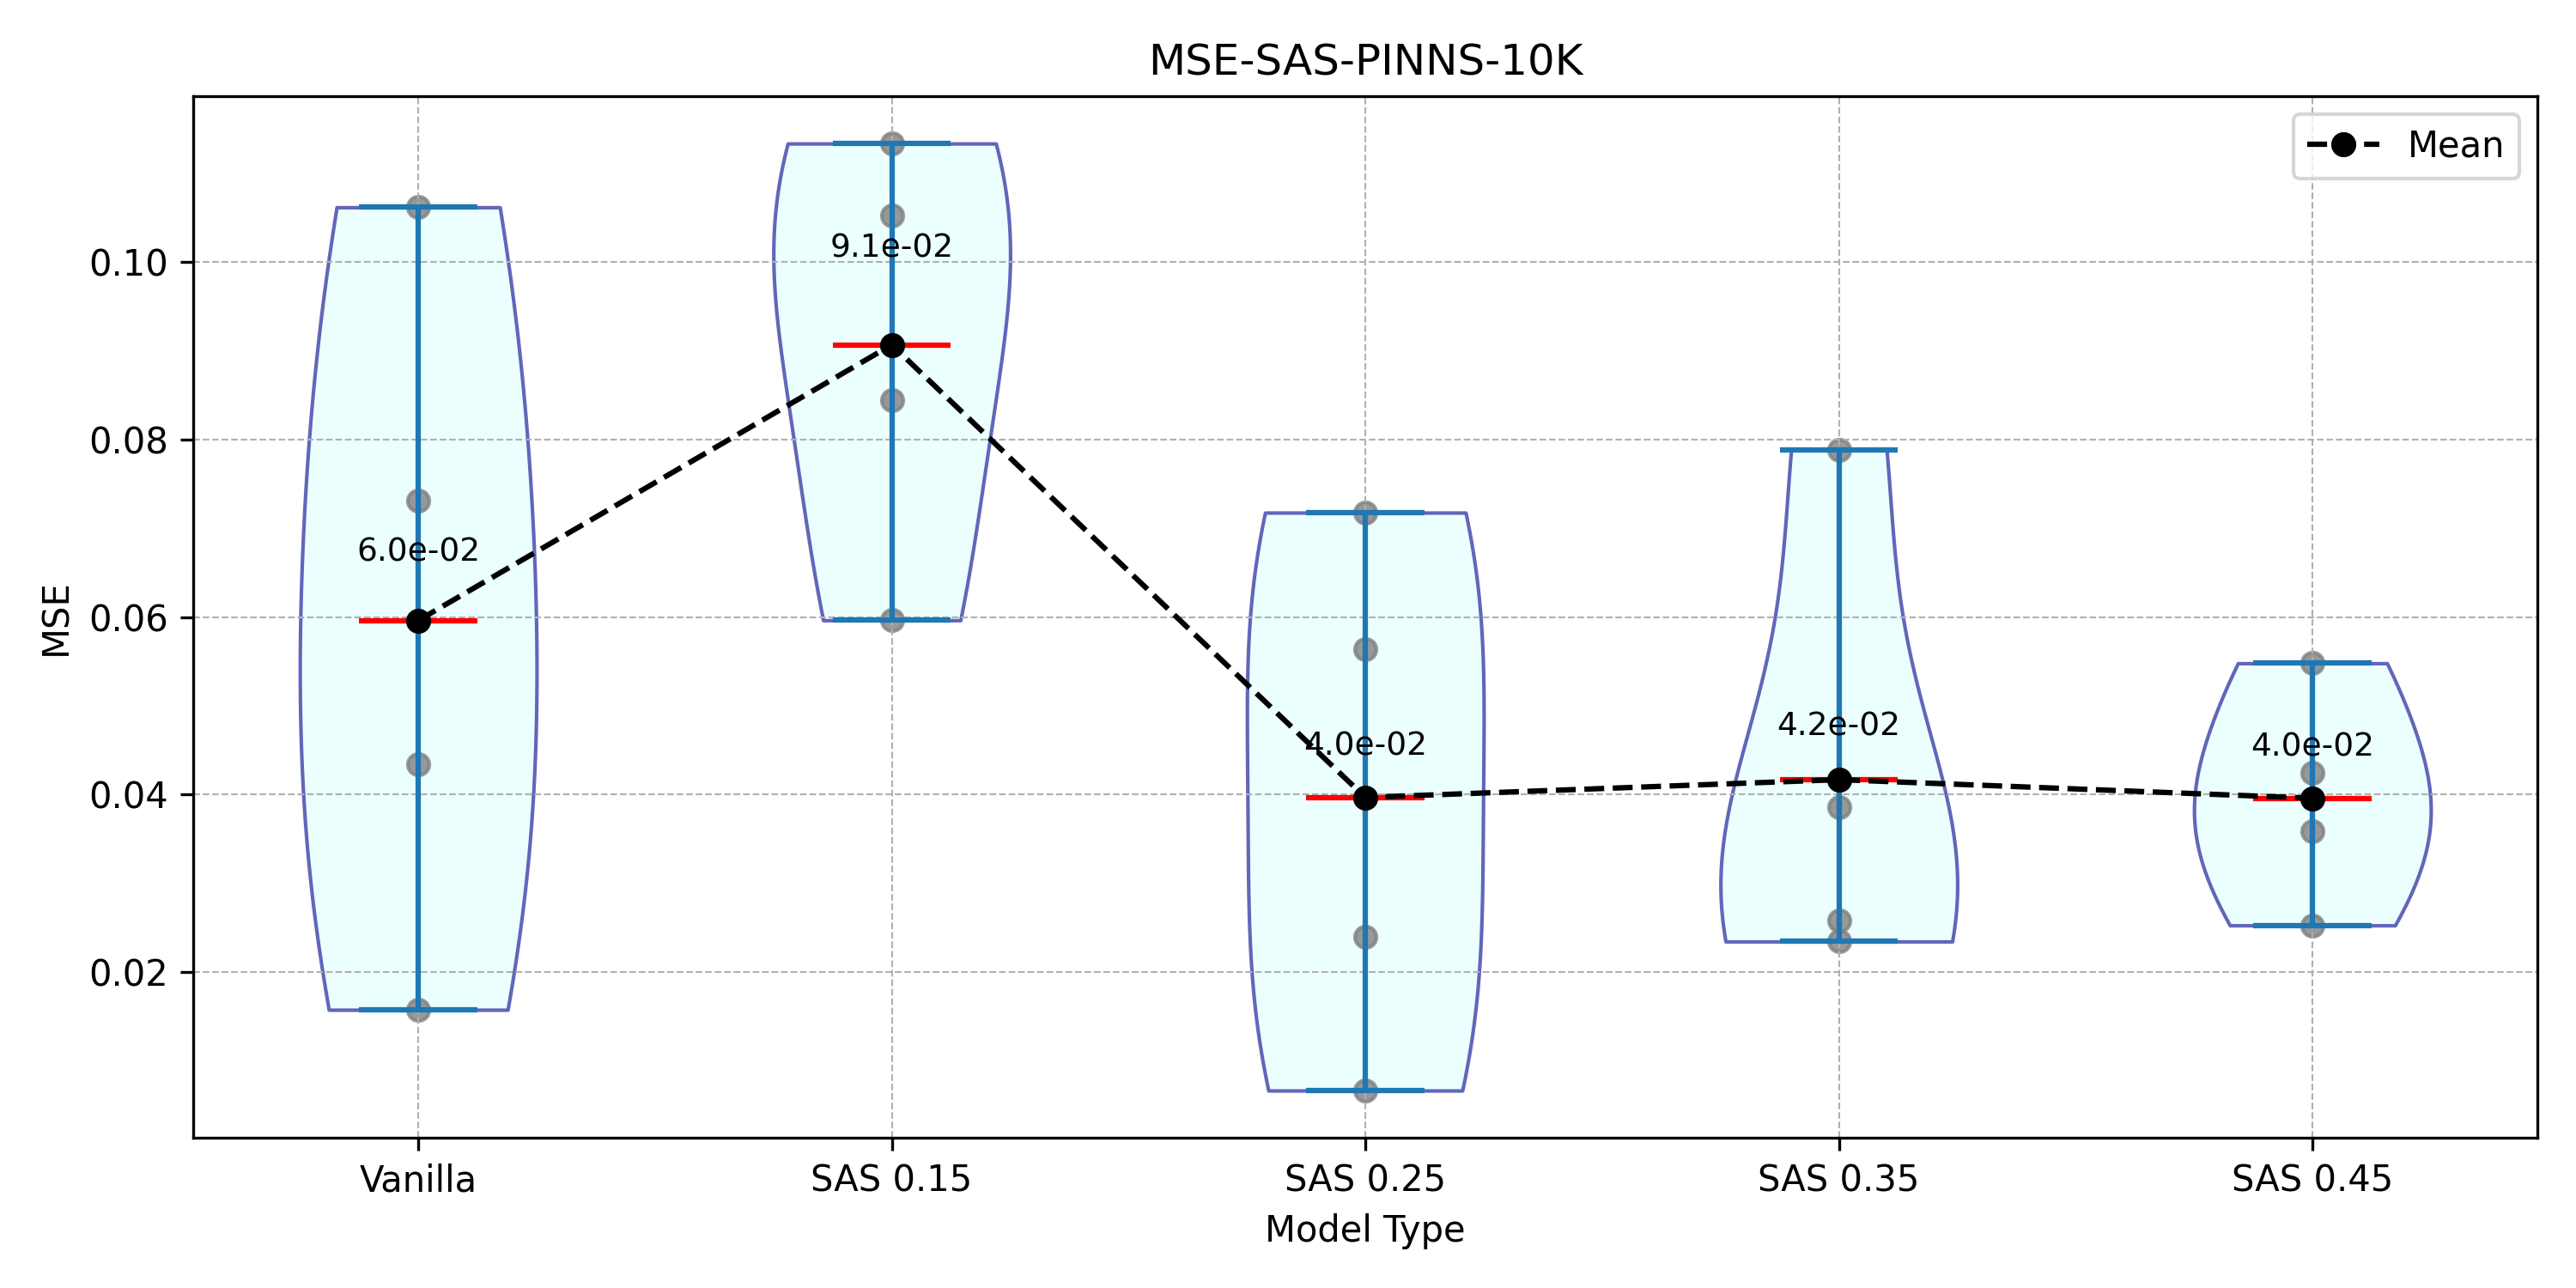
\includegraphics[width=1 \linewidth]{Gambar/smoteDistribution-All.png}
    \caption{Perbandingan MSE Vanilla-PINNs vs SAS-PINNs}
    \label{fig:Good-SAS-PINNs}
\end{figure}

Evaluasi MSE SAS-PINNs diberikan pada Gambar \ref{fig:Good-SAS-PINNs}. Model SAS-PINNs dibandingkan dengan model Vanilla-PINNs yang dilatih pada sampel kolokasi yang sama sejumlah 10.000 titik. Rata-rata MSE dari model Vanilla berada pada angka 0.06. Model SAS-PINNs pada nilai ambang 0.25--0.45 berdasarkan konfigurasi \ref{SAS-config} menunjukkan penurunan pada angka MSE rata-rata, masing-masing yakni, 0.04, 0.042, dan 0.04. Akan tetapi, pada nilai ambang 0.15, nilai MSE rata-rata justru meningkat menjadi 0.091.


\begin{figure}[htbp]
    \centering
    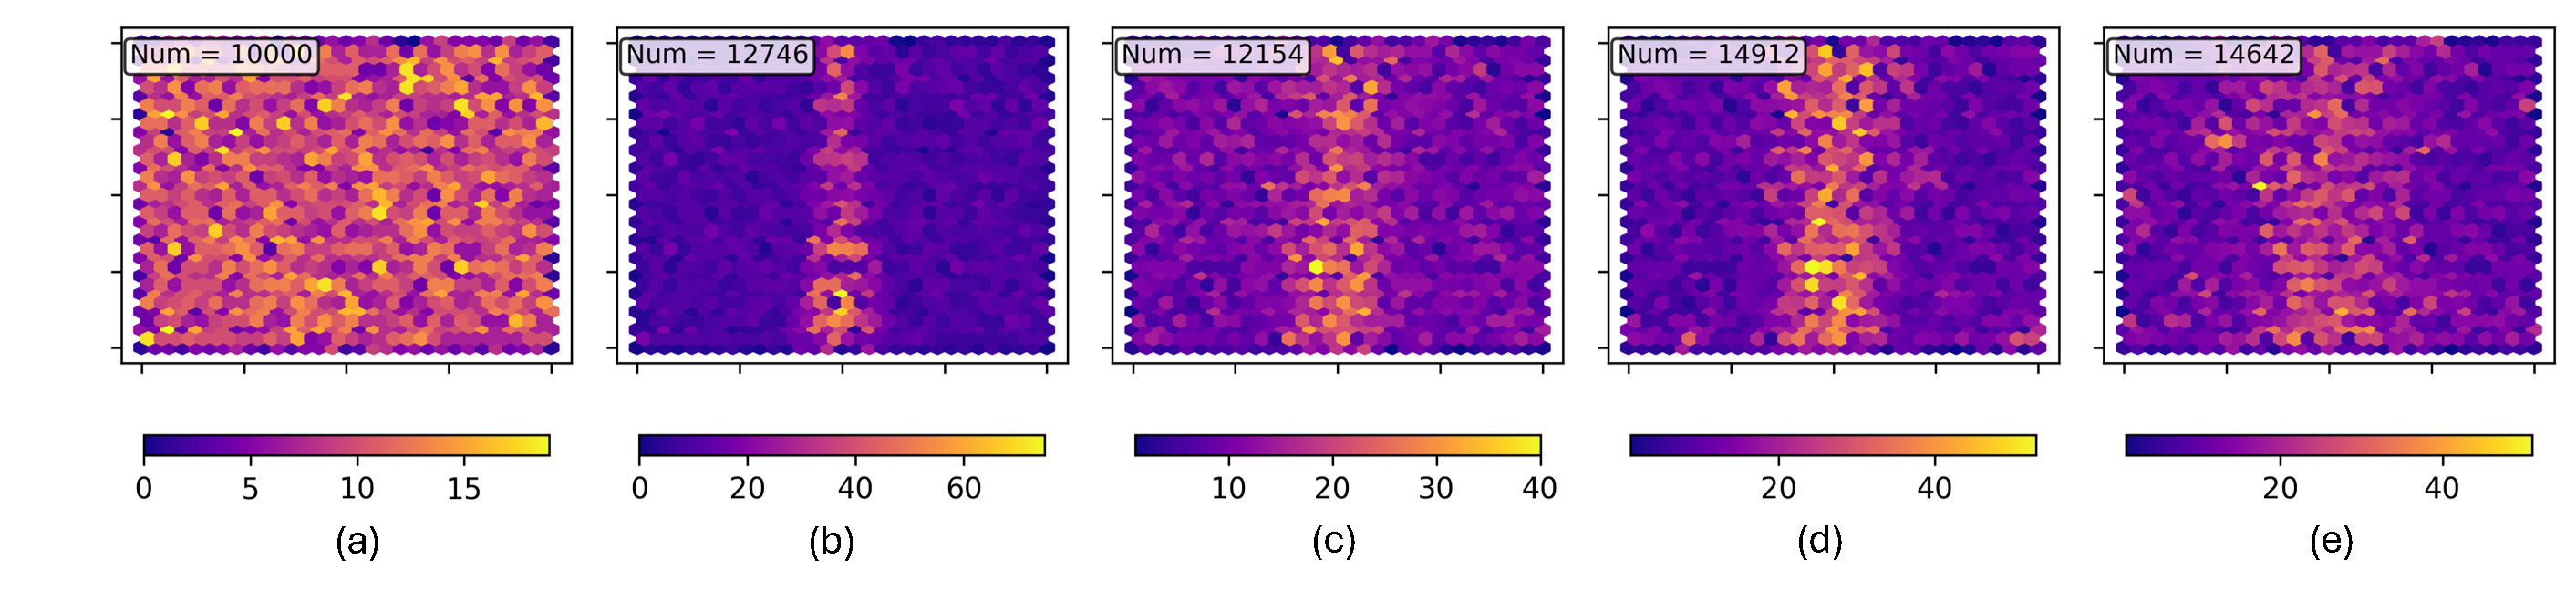
\includegraphics[width=1 \linewidth]{Gambar/colSMOTE.png}
    \caption{Distribusi Sampel SAS-PINNs Terkonfigurasi}
    (a) Titik Kolokasi Vanilla-PINNs; (b)-(e) Titik Kolokasi SAS-PINNs pada Keempat Tipe Konfigurasi Tabel \ref{SAS-config}
    \label{fig:col-SAS-PINNs}
\end{figure}

Konfigurasi nilai ambang 0.15 memberikan augmentasi titik yang terfokus. Walaupun hanya sejumlah 2.746 titik yang ditambahkan, kawasan penambahan titik yang terlalu terpusat pada 15\% zona residual tertinggi terbukti berdampak buruk terhadap konvergensi PINNs. Di lain sisi, penambahan titik dengan jumlah yang serupa (2.154 titik) pada 25\% zona residual tertinggi justru mampu memperbaiki konvergensi model. Sementara itu, pengaturan nilai ambang 0.45 memberikan persebaran titik tambahan yang lebih luas, tetapi menghasilkan presisi terbaik dari model SAS-PINNs yang lain. 

Dapat disimpulkan bahwa strategi penambahan titik yang paling optimal didapatkan ketika nilai ambang SAS-PINNs cukup besar. Hal ini menyebabkan penambahan titik dilakukan pada area yang lebih luas. Penambahan selektif ini memungkinkan model memfokuskan kapasitasnya pada daerah tertentu, dengan tetap menjaga cakupan global domain fisis. Akan tetapi, nilai ambang yang terlalu kecil berpotensi membuat model terlalu selektif sehingga kehilangan informasi penting dari domain lainnya. 

Hal ini dibuktikan pada Gambar \ref{fig:loss-SAS-PINNs}, di mana penambahan titik kolokasi menyebabkan nilai loss meningkat secara periodik setiap 10.000 epoch. Akan tetapi, pada strategi nilai ambang sampling 0.15, peningkatan periodik ini menjadi sangat signifikan sehingga konvergensi proses pembelajaran menjadi stagnan. Akibatnya, pada proses optimasi L-BFGS, model tidak dapat melakukan konvergensi sebaik model SAS-PINNs dengan nilai ambang 0.45, maupun dengan model Vanilla-PINNs.

\begin{figure}[htbp]
    \centering
    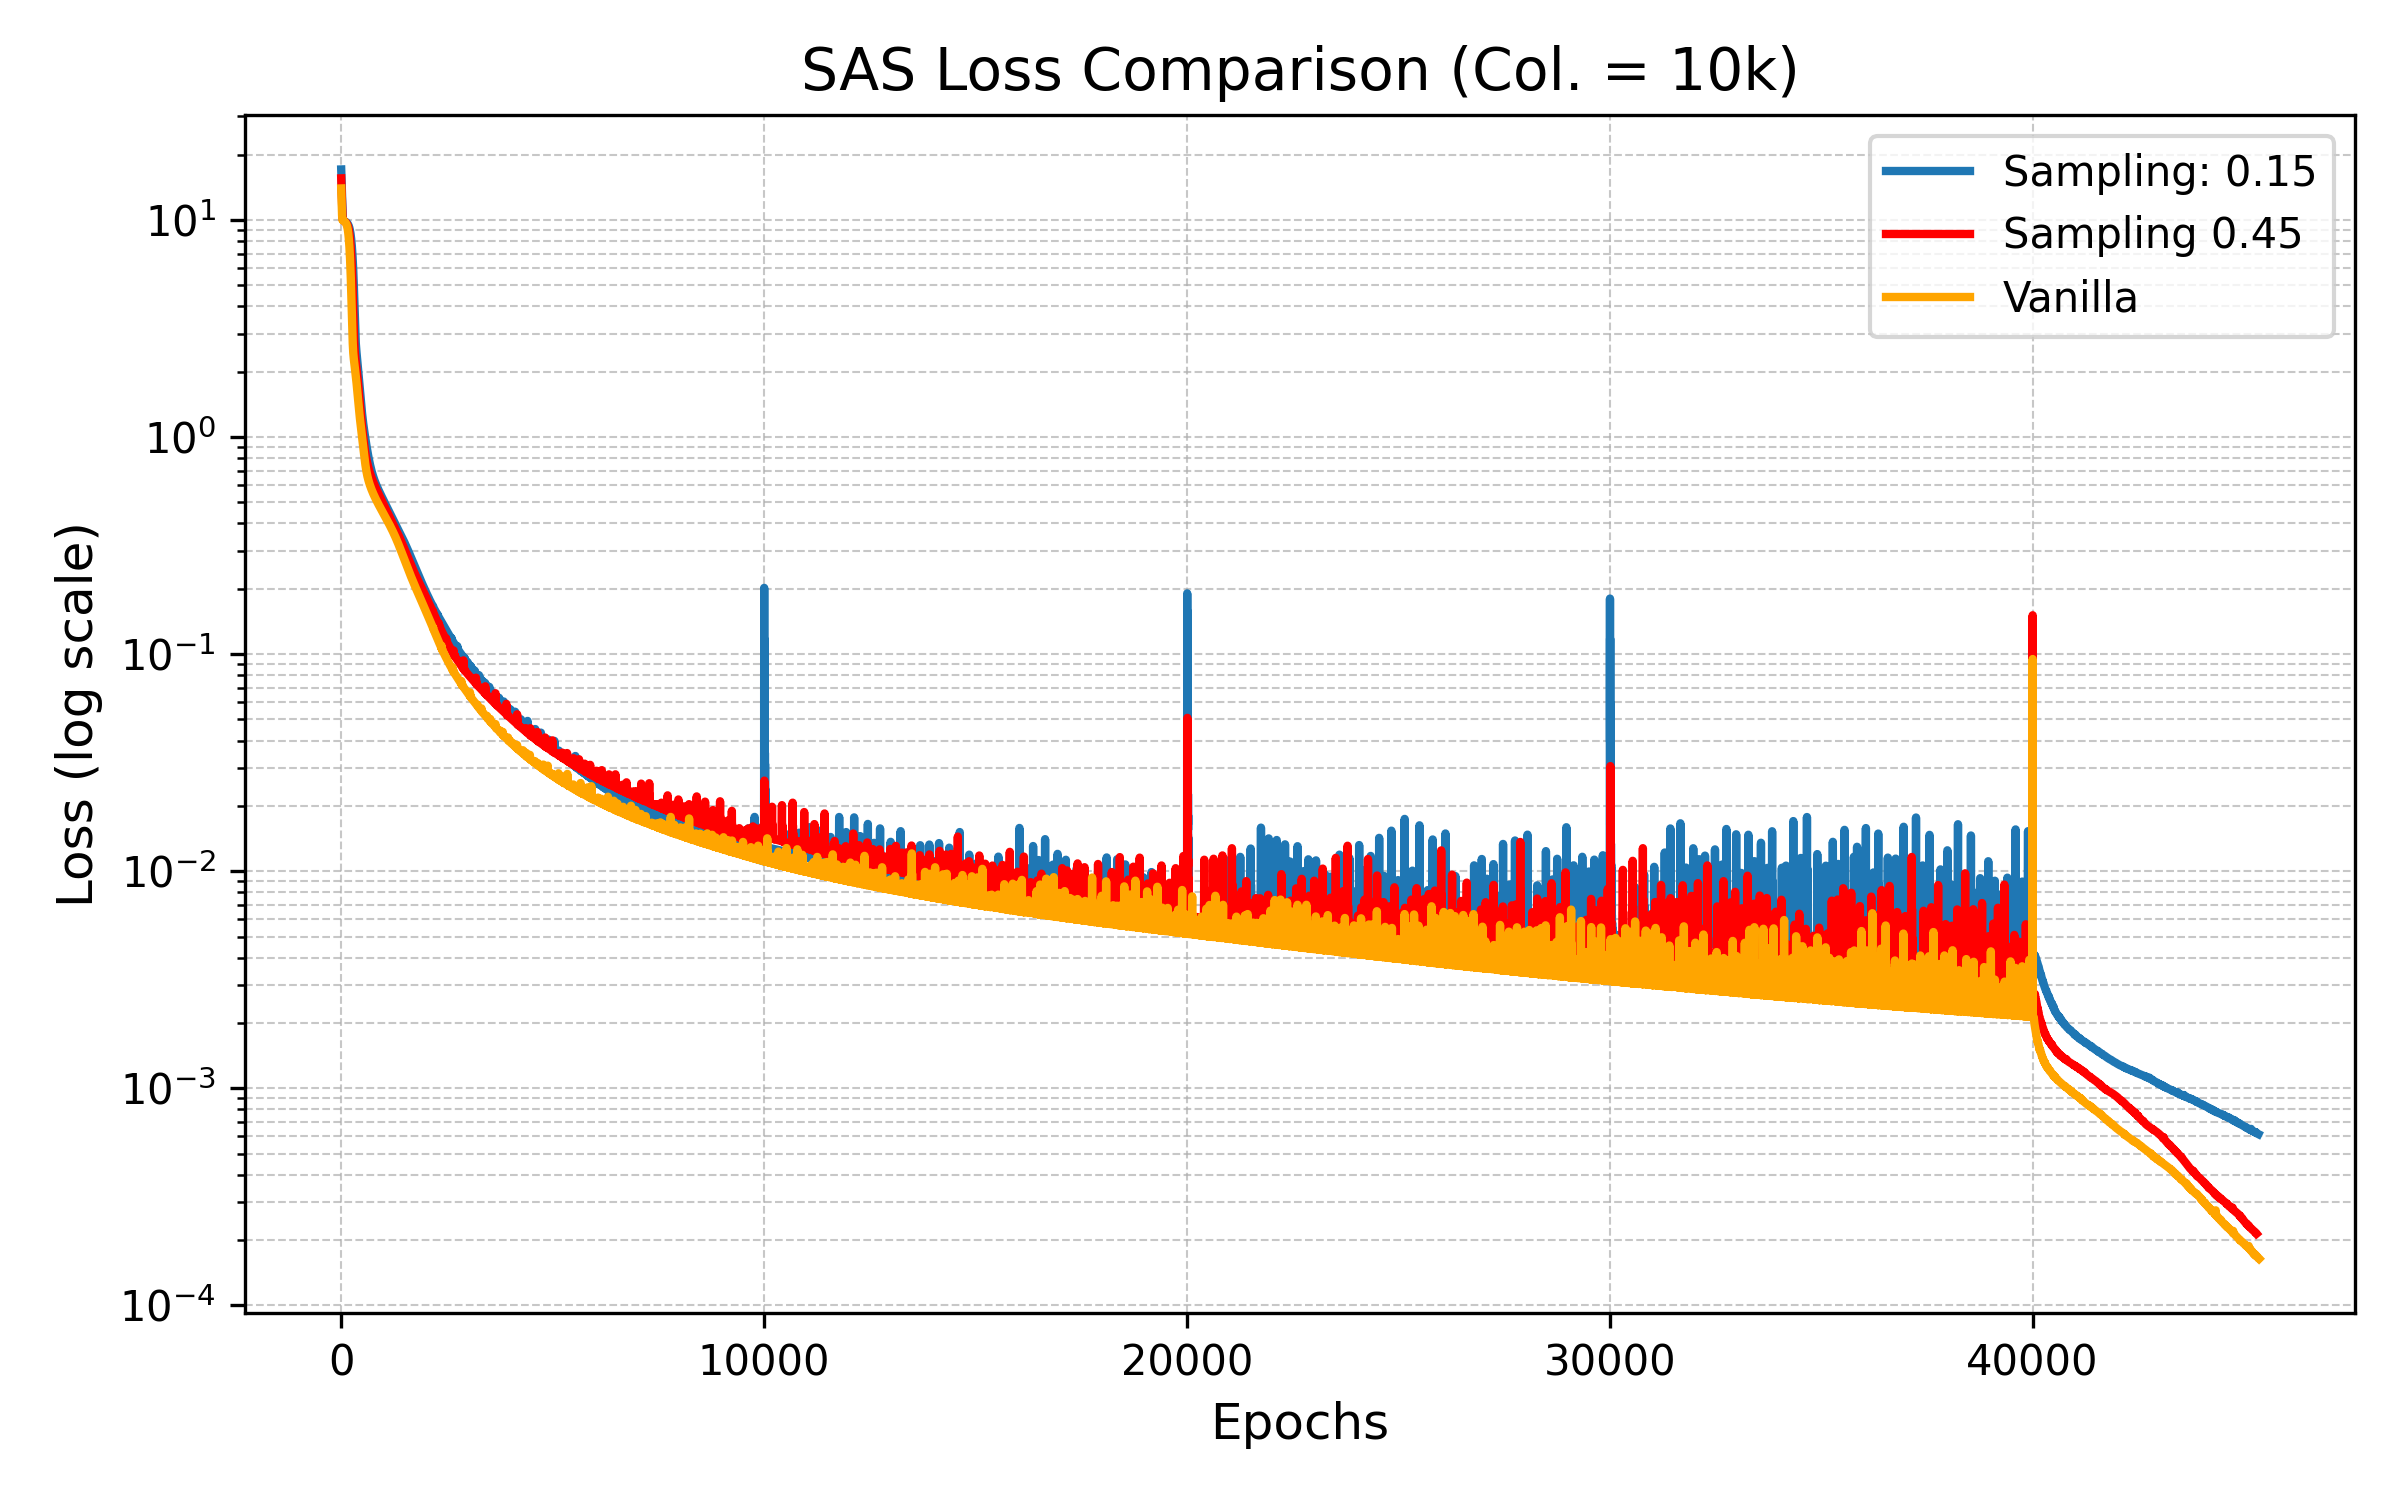
\includegraphics[width=0.8 \linewidth]{Gambar/SASLoss-Comparison (1).png}
    \caption{Perbandingan Konvergensi Loss Model}
    \label{fig:loss-SAS-PINNs}
\end{figure}

%%%%%%%%%%%%%%%%%%%%%%%%%%%%%%%%%%%%%%%%%%%%%%%%%%%%%%%%%%%%%%
\cleardoublepage